\documentclass{article}
\usepackage[utf8]{inputenc}
\usepackage{notoccite}
\usepackage{graphicx}
\usepackage{authblk}



\title{INDIGO-DataCloud: Project Achievements}



\author[ ]{\large by the {{\bf INDIGO-DataCloud Collaboration} \\}} 

% Management
\author[1]{\small{\\ D. Salomoni}}
\author[2]{I. Campos}
\author[3]{L. Gaido}

%WP leaders / deputies in WP order
\author[2]{J. Marco de Lucas}
\author[14]{P. Solagna}
\author[9]{J. Gomes}
\author[13]{L. Matyska}
\author[5]{P. Fuhrman}
\author[8]{M. Hardt}
\author[4]{G. Donvito}
\author[13]{L. Dutka}
\author[7]{M. Plociennik}
\author[11]{R. Barbera}

% Task leaders alphabetic
\author[1]{C. Aiftimiei}
\author[6]{I. Blanquer}
\author[1]{A. Ceccanti}
\author[9]{M. David}
\author[2]{A. L\'opez-Garc\'{\i}a}
\author[6]{G. Molt\'o}
\author[2]{P. Orviz}
\author[13]{Z. Sustr}
\author[14]{M. Viljoen}



% Rest in alphabetic order
\author[2]{F. Aguilar}
\author[9]{L. Alves}
\author[16]{A. Bonvin}
\author[11]{R. Bruno}
\author[18]{D. Davidovic}
\author[8]{B. Ertl}
\author[11]{M. Fargetta}
\author[14]{Y. Chen}
\author[10]{S. Fiore}
\author[16]{Z. Kurkcuoglu}
\author[2]{L. Lloret}
\author[9]{J. Martins}
\author[10]{A. Nuzzo}
\author[10]{P. Nassisi}
\author[9]{J. Pina} 
\author[17]{E. Sciacca}
\author[12]{D. Spiga}
\author[4]{M. Tangaro}
\author[7]{M. Urbaniak}
\author[8]{B. Wegh}
\author[7]{T. Zok}




{\small {

\affil[1]{\small{INFN Division CNAF (Bologna), Italy}}
\affil[2]{IFCA, Consejo Superior de Investigaciones Cientificas-CSIC, Santander (Spain)}
\affil[3]{INFN Division of Torino, Italy}
\affil[4]{INFN Division of Bari, Italy}
\affil[5]{Deutsches Elektronen Synchrotron (DESY), Germany}
\affil[6]{Universitat Polit\`ecnica de Valencia, Spain}
\affil[7]{PSNC IBCh PAS, Poland}
\affil[8]{Karlsruhe Institute of Technology (KIT), Germany}
\affil[9]{Laboratory of Instrumentation and Experimental Particle Physics (LIP), Portugal}
\affil[10]{Fondazione Centro Euro-Mediterraneo sui Cambiamenti Climatici , Lecce, Italy}
\affil[11]{INFN Division of Catania, Italy}
\affil[12]{INFN Division of Perugia, Italy}
\affil[13]{Cyfronet AGH, Krakow, Poland}
\affil[14]{European Grid Initiative Foundation, EGI.eu, Amsterdam (Netherlands)}
\affil[15]{CESNET, Prague, Czech Republic}
\affil[16]{University of Utrecht, The Netherlands}
\affil[15]{Istituto Nazionale di Astrofisica, Italy}
\affil[15]{Ruder Boskovic Institute, Zagreb (Kroatia)}
}}


\begin{document}

\maketitle

\begin{abstract}
This paper describes the achievements of the H2020 project INDIGO-DataCloud. The project has provided  e-infrastructures  with  tools, applications and cloud framework enhancements to manage the demanding requirements of scientific   communities,   either   locally   or through enhanced  interfaces. The middleware developed allows to federate hybrid resources, to easily write, port and run scientific applications to the cloud. Our developments are freely downloadable as open source components, and are already being integrated into many scientific applications.
\end{abstract}

\newpage

\tableofcontents

\newpage

\section{Introduction}

INDIGO-DataCloud was an European project starting in April 2015, with the
purpose of developing a modular architecture and software components to improve
how scientific work is supported at the edge of computing services development.
Its main goal has been to deliver a Cloud platform addressing the specific
needs of scientists in a wide spectrum of disciplines, engaging public
institutions and private companies. It aimed at being as inclusive as possible,
developing open source software exploiting existing solutions, adopting and
enhancing state of the art technologies, connecting with other initiatives and
with leading commercial providers.

Since its inception, the project roadmap has been user community driven. Its
main focus was on closing the existing technology gaps that hindered an
optimal exploitation of Cloud technologies by scientific users. In order to do
so, user requirements from several multidisciplinary scientific communities
were collected, and systematized into specific technical requirements. This
process was carried out across the entire lifetime of the project, which
allowed the update of existing requirements as well as the insertion of new
ones, thus driving the project architecture definition and the technological
developments.

The project also made focus on delivering production-quality software, thus it
defined procedures and quality metrics, which were followed by, and
automatically checked for, all the INDIGO components. A comprehensive process
to package and issue the INDIGO software was also defined. As an outcome of
this, INDIGO delivered two main software releases (the first in August 2016,
the second in April 2017), each followed by several minor updates. The latest
release consists of about 40 open modular components, 50 Docker
containers, 170 software packages, all supporting up-to-date open operating
systems. This result was accomplished reusing and extending open source
software and ---whenever applicable--- contributing code to upstream projects.

The paper is structured as follows.
Section~\ref{sec:user-req} contains a description on how the user requirements
were collected and consolidated. From there, the INDIGO architecture is further
elaborated from the lower Infrastructure as a Service layer
(Section~\ref{sec:iaas}) moving towards the Platform layer
(Section~\ref{sec:paas}) in order to arrive to the user interfaces
(Section~\ref{sec:users}). The overall software development process is
described in Section~\ref{sec:release}. Section~\ref{sec:examples} contains a
summary of some usage patterns on how to leverage the INDIGO solutions to
develop, deploy and support applications in a Cloud framework. The conclusions
are laid out in Section~\ref{sec:conclusions}. The list of upstream contributed
software can be found in the Appendix.

\subsection{Context and state of the art}


From the collection of user community requests, and its consolidation into technical requirements (see section \ref{sec:user-req}), we identified a number of technology gaps that today hinder an optimal scientific exploitation of heterogeneous e-infrastructures.

In this Section we will elaborate more on the general strategy to address those requirements, linking our developments with the previous and existing works. The specific enhancements and developments will be further elaborated in the corresponding sections.

Lack of proper federated identity support across several e-Infrastructures is a key issue for the reseachers perspective. The provision of an effective distributed authentication and authorization in heterogeneous platforms is fundamental to support access to distributed infrastructures. Several efforts have been made in this context
\cite{LopezGarcia2013b,Chadwick2014,lee2014design,pustchi2015authorization,lee2014keystone}
but they were focused on specific infrastructures and services. However,
although some of these approaches have been used in production in specific
e-Infrastructures \cite{FernandezdelCastillo2015} they are difficult 
to implement in a broader environment. 

In parallel to the development of INDIGO-Datacloud, the
{\sl Authentication and Authorisation for Research and Collaboration} project (AARC)
defined the AARC Blueprint Architecture \cite{aarc}. This document describes a 
set of interoperable architecture building blocks for designing and implementing access management
solutions for international research collaborations. Following the AARC recommendations we have
developed several key components related with identity and access management,
providing a framework compliant with the proposed blueprint architecture, as
will be described in Section~\ref{sec:iam}.

Facilitating the transparent execution of user applications across different
computing infrastructures is also a key issue \cite{Oesterle2015}. 
Advanced users have nowadays at their disposal tools to implement 
applications in Clouds provisioned in {\sl Infrastructure as a Service} (IaaS) mode. 
Examples of such solutions are virtual appliances and contextualization \cite{Campos2013} or 
container technologies \cite{boettiger2015introduction}). 

The situation for non-Cloud resources in scientific facilities is completely different.
Here we are referring for instance to local clusters, Grid infrastructures and HPC systems. 
Such infrastructurs are tipycally shared among many users with different requirements, therefore 
it is managerially and technically impossible offering tailored environments to all of them.
As a consequence scientific users often need to follow a troublesome process to package and 
execute their applications. 

To address this problem we have applied the technology of Docker containers \cite{DOCKER} to facilitate applications execution in multiuser environments. As a result we have provided a flexible user-level solution to provide autonomy to users in shared computing facilities \cite{udocker-paper}. Section \ref{sec:containers} contains a thorough discussion on the strategy and outcomes.

Adoption of true Platform as a Service (PaaS) Cloud solutions is a common problem for
scientific communities. The roots of this problem are on the one hand the non-interoperability of the interfaces \cite{Zhang2013,Lorido-Botran2014}, and second, the lack of true orchestration
mechanisms across federated heterogeneous infrastructures. Both barriers made it difficult 
for users to adopt Cloud hybrid solutions.

In Section~\ref{sec:paas} we describe our approach, and how we have tackled this problem by 
leveraging the OCCI \cite{Nyren2010,Metsch2010,Metsch2011} and TOSCA \cite{TOSCA} open
standards. In this regard we have not only supported those standards at the
corresponding architectural levels \cite{Teckelmann2011,LopezGarcia2016b}, but
also we made important contributions to both the standards specifications and
implementations. INDIGO has contributed to the networking parts of the OCCI
standard, as well as to the improvement of the TOSCA support in the upstream OpenStack
components: the Heat Translator and TOSCA parser \cite{LopezGarcia2017b}. Our solution makes the execution of dynamic workflows \cite{Hardt2012,Fakhfakh2014,Stockton2017} possible, in more consistent way across hybrid Clouds \cite{PLOCIENNIK2016722}.

In this interoperability context, hybrid Cloud deployments, although possible
\cite{moreno2011multicloud,Katsaros,Lorido-Botran2014}, were complicated from a practical 
point of view and therefore user adoption has been hindered. 
By adopting INDIGO solutions users can now express their requirements and deploy them as applications over those hybrid infrastructures \cite{LopezGarcia2017}. 

Linked with the previous statements another outstanding gap was the lack of
advanced scheduling features in Cloud environments
\cite{Singh2016}. Common cloud usage scenarios, being industry driven, do not
take into account the unique requirements of scientific applications
\cite{LopezGarcia2017c}, leading to an inefficient utilization of the resources
or to non optimal user experience. 

Developments in this area can be found in the literature 
\cite{Chauhan2017,Somasundaram2014,Sotomayor2006,Manvi2014}, where it becomes evident that 
there are many challenges to be addressed. Within INDIGO we focused
(see Section~\ref{sec:sched}) in the efficient sharing of resources between users
following fair-share approaches (limiting the amount of resources that can be
consumed by a user group), proper quota partitioning across different computing
frameworks (like HPC and Cloud resources) or new Cloud computing execution
models (like preemptible instances) as these are aspects hat affect both users
and resource providers.

Regarding storage support, INDIGO has performed substantial contributions to
storage-related entities and standardization bodies, such as the Research Data
Alliance (RDA), where INDIGO has been highly involved the Quality of Service,
Data Life cycle and Data Management Plans working group (now renamed to Storage
Service Definitions). Moreover, INDIGO has also contributed this work to the
SNIA CDMI standard, providing several extensions that have been included in
SNIA reference implementations and documents.



%%%%%%%% NEW TEXT ISABEL %%%%%%%%%%%%%%%



\section{Analysis of requirements coming from research communities}
\label{sec:user-req}

In order to guide our developments we performed an analysis of a number of use cases originating in several flagship research communities. In particular coming from the areas of High Energy Physics, Environmental modelling, Bioinformatics, Astrophysics and Social sciences. See Table \ref{tab:req} for the full list.



% Here goes table from page 21 of the deliverable D2.1 slightly enhanced

\begin{table}
  \centering
  \begin{tabular}{c|p{9cm}}
    {\bf Research community} & {\bf Application/Use Case} \\ \hline \hline
 \\   LIFEWATCH (Biodiversity) & {\bf Monitoring and Modelling Algae Bloom in a Water Reservoir:} Support of hydrodynamic and water quality modelling including data input-output management and visualization. \\ \hline
 \\   INSTRUCT (Bioinformatics) &  {\bf Molecular dynamics simulations:} Support of Molecular dynamics simulations of macromolecules that need specific hardware (GP/GPUs) using a pipeline of software that combines protocols that automate the step for setup and execution of these simulations.  \\ \hline
 \\   CTA (Astronomical Data) & {\bf Astronomical Data Archives:} Data analysis and management using different tools such as data discovery, comparison, cross matching, data mining and also workflows. The use case could be described as follows: data production, data reduction, data quality, data handling and workflows, data publication and data link to articles   \\ \hline
 \\   Climate Modelling &  {\bf Intermodel comparison} of data analysis for different climate models \\ \hline
 \\   EuroBioImaging (Bioinformatics) & {\bf Medical Imaging Biobanks:} The virtual Biobank integrates medical images from different sources and formats. This case study includes all the steps needed to manage the images, like analysis, storage, processing (pre, post). Privacy is a constraint to take into account for user management \\ \hline
 \\   ELIXIR (Bioinformatics) & {\bf Galaxy as a Cloud service:} Deployment of Galaxy instance that should support all the software/steps needed by the pipeline over, for example, a virtual cluster or cloud instances. \\ \hline
 \\   DARIAH (Social Sciences) & Transparent access to data catalogues and on-demand data management features. \\ \hline
 \\   Mastercode (HEP Pheno) & {\bf Complex combination of codes including legacy parts} to perform combined analysis of data coming from particle detectors, astrophysics experiments, and dark matter detectors. Installation of these codes is in general very complex in multi-user farms. Providing a container based solution would simplify installation across infrastructures. \\ \hline
 \\   Lattice QCD  (HEP) & Lattice simulations run on large HPC facilities using low latency interconnects, producing large amounts of output. Accessing such facilities in Cloud mode would require implementing {\bf MPI parallel processing capabilities}. \\ \hline
  \end{tabular}
  \caption{Research Communities and use cases analyzed to extract general requirements}
  \label{tab:req}
\end{table}


The deployment of customized computing back-ends, such as batch queues, including automatic elasticity is among the features more demanded by researchers. The automation of the deployment of user-specific software in VMs or containers is also on the top of their wish list. Such automation is a {\sl must} when it is about simplifying the executing applications in heteregenous infrastructures. For similar reasons, highly specialized applications require also support to hardware accelerators and specialized hardware such as Infiniband, multicore systems, or GP/GPUs.

Often user communities are asking about terminal access to resources, workflow management and data handling, in a way that such access is linked to a common Authorization and Authentication Infrastructure. 

In order to generalize the requirements, we have extracted two generic usage scenarios, which can support a wide range of applications in these areas. The first generic use case is computing oriented, while the second is data analysis oriented. For full details regarding user communities description and detailed usage patterns we refer to the users requirements deliverable of the project available publicly in \cite{D21}.



\subsection{Computing Portal Service}

The first generic user scenario is a computing portal service. In such scenario, computing applications are stored by the application developers in repositories as downloadable images (in the form of VMs or containers). Such images can be accessed by users via a portal, and require a back-end for execution; in the most common situation this is typically a batch queue. Support for parallel processing using containers is a requeriment that comes up as well from the users.

The application consists of two main parts: the portal / Scientific Gateway and the processing working nodes. The number of nodes available for computing should increase (scale out) and decrease (scale in), according to the workload. The system should also be able to do Cloud-bursting to external infrastructures when the workload demands it. Furthermore, users should be able to access and reference data, and also to provide their local data for the runs. A solution along these lines is shown in Figure \ref{fig:01}.

\begin{figure}
  \centering
  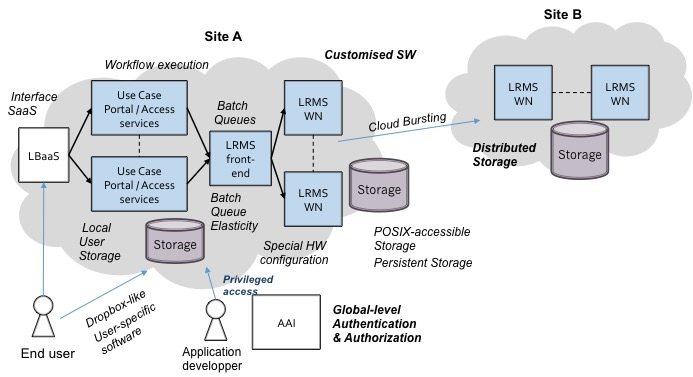
\includegraphics[width=11cm]{./figs/Figure01.jpg}
  \caption{User Community Computing Portal Service}
  \label{fig:01}
\end{figure}

A solution along these lines has been requested in the user scenarios coming from ELIXIR, WeNMR, INSTRUCT, DARIAH, Climate Change and LIFEWATCH.

\subsection{Data Analysis Service}

A second generic use case is described by scientific communities that have a coordinated set of data repositories and software services to access, process and inspect them. 

Processing is typically interactive, requiring access to a console deployed on the data premises. The application consists of a console / Scientific Gateway that interacts with the data. In Figure \ref{fig:02} we show a schematic view of such a use case. Examples of such include {\sl R}, {\sl Python} or {\sl Ophidia}. It can be a complementary scenario to the previous one, and it could also expose programmatic services.

The communities related to INSTRUCT, CTA, Climate Change, LIFEWATCH and Lattice QCD have requested related features.

\begin{figure}
  \centering
  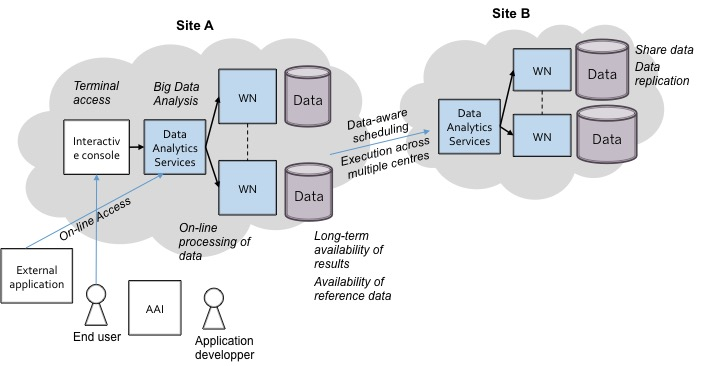
\includegraphics[width=11cm]{./figs/Figure02.jpg}
  \caption{Data Analysis Service}
  \label{fig:02}
\end{figure}


%%%%%%%%%%%%%%%%%%%%%%%%%%%%%%%%%%%%%%%%%%

\section{Developing for the Infrastructure as a Service (IaaS) Layer}
\label{sec:iaas}

INDIGO-DataCloud  has  provided  e-infrastructures  with  tools, applications and cloud framework enhancements to manage the demanding requirements of modern scientific   communities,   either   locally   or through enhanced  interfaces enabling those infrastructures  to  become  part  of  a  federation  or to connect  to  federated  platform  layers (PaaS). 

In this section we will describe the highlights of this development work, which was needed to properly interface with the resource centers. This work has focussed on virtualizing local compute, storage and networking resources (IaaS) and on providing those resources in a standardized, reliable and performing way to remote customers or to higher level federated services, building virtualized site independent platforms.

The IaaS resources are provided by large resource centers, typically engaged in well-established European e-infrastructures. The e-infrastructure management bodies, or the resource centers themselves will select the components they operate, and INDIGO will have limited influence on that process. 

Therefore, INDIGO has concentrated on a selection of the most prominent exisitng components and has further developed the appropriate interfaces to high-level services based on standards. We have also developed new components where we felt a full functionality was completely missing. Figure \ref{fig:1} shows a very schematic view of the interrelation among those components.



\begin{figure}
  \centering
  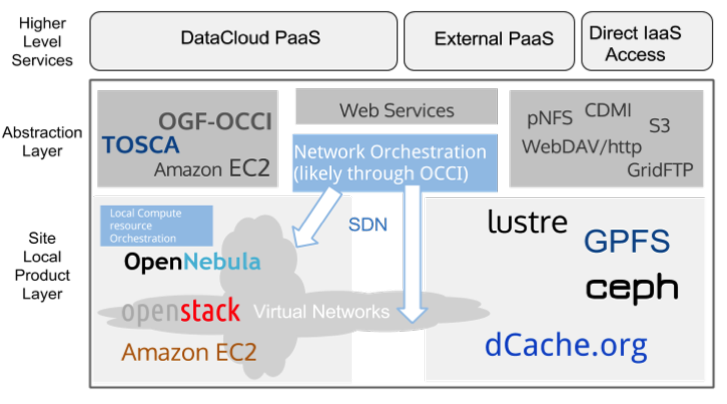
\includegraphics[width=\textwidth]{./figs/Figure1.pdf}
  \caption{Components at the Infrastructure as a Service level and their relation with the INDIGO developments}
  \label{fig:1}
\end{figure}



The contribution of INDIGO to enhance the flexibility to access resources in Cloud and HPC infrastructures will be of paramount  importance to  enable  transparent  execution  of  applications  across  systems promoting the development of the future European Open Science Cloud (EOSC) ecosystem \cite{EOSC}.

As we describe below new components  are  provided,  or already  existing  components  are improved  in  the areas   of   computing,   storage,   networking and Authorization and Authentication Infrastructure (AAI).   For   almost   all   components, we succeeded in committing modifications to the corresponding upstream software providers and by that, significantly contributed to  the  sustainability  model  of  the  software.

\subsection{Supporting Linux containers}
\label{sec:containers}

INDIGO  has  provided  support  for  container  execution, both  interactively  and  through  batch systems,  in cloud and conventional clusters. This was achieved by developing new tools and extending existing ones.
 
The key middleware developed for this purpose is {\bf udocker}\cite{udocker-paper}\footnote{https://github.com/indigo-dc/udocker}. The udocker novelty consists in enabling pull and execution of Docker containers \cite{DOCKER} without using or requiring the installation of the Docker software. By using udocker it is possible to encapsulate applications in Docker containers and execute them in batch or interactive systems where Docker is unavailable. It provides several different execution engines based on PRoot\cite{PROOT}, runC\cite{RUNC} and Fakechroot\cite{FAKECHROOT}. None of the udocker engines requires root privileges for installation or execution being therefore adequate for deployment and use by end-users without system administrator intervention. In addition the PRoot and Fakechroot engines execute containers via pathname translation and therefore do not require the use of Linux namespaces. 

Since udocker never requires privileges and executes as unprivileged user many of the security concerns associate with the Docker software are avoided. Udocker also supports GPGPU and MPI applications, making it adequate to execute containers in batch systems and HPC clusters. The udocker software suite is meant to be easily deployed by end-users. It only requires the download and execution of a Python script to quickly setup udocker within the user home directory. Udocker empowers end-users to execute Docker containers regardless of the Linux host environment.

Since its first release in June 2016 udocker expanded quickly in the open source community. It has been adopted by a number software projects as a drop-in replacement for Docker. Among them openmole, bioconda, common-work language (cwl)  or SCAR - Serverless Container-aware ARchitectures\cite{Perez2018scc}.

As an example, udocker  is  being  used  with  great  success  to  execute  code  produced  by  the  MasterCode collaboration\cite{MASTERCODE}.   The   MasterCode   collaboration   is   concerned   with   the   investigation of Supersymmetric  models  that  go  beyond  the  current  status  of  the  Standard  Model  of  particle physics.  It  involves  teams  from  CERN,  DESY,  Fermilab,  SLAC,  CSIC,  INFN,  NIKHEF, Imperial College   London,   King's   College   London,   the   Universities   of   Amsterdam, Antwerpen, Bristol, Minnesota and ETH Zurich. Examples and documentation can be found at https://github.com/indigo-dc/udocker.

INDIGO has also developed {\bf bdocker}\footnote{https://github.com/indigo-dc/bdocker}, which provides a front-end to execute the Docker software in batch systems under restrictions and limits configurable by the system administrator (resource consumption, access to host directories, list of container images, etc). It has been implemented for the SoGE (Son of Grid Engine) batch system but can be extended to other batch systems. This integrates the benefits of application delivery provided by Docker with the scheduling policies of the batch system. While udocker can be deployed directly by the end-user, bdocker is installed and configured by the system administrator to provide the users with the ability to run limited execution environments provided by Docker. Finally, ONEDock\footnote{https://github.com/indigo-dc/onedock} was developed to introduce support to the execution of containers as if they were Virtual Machines in OpenNebula-based on-premises Clouds, by supporting Docker as a hypervisor in this Cloud Management Platform.

\subsection{Development of advanced Scheduling Technologies}
\label{sec:sched}

INDIGO pushed the  state  of  the  art  in  scheduling  technologies  by  implementing  preemptible instances  on  top  of  the  OpenStack\cite{OPENSTACK}  cloud  management  framework, {\bf opie}\footnote{https://github.com/indigo-dc/opie}. Openstack preemptible instances is the materialisation of the preemptible instances extension, serving as a reference implementation.

Preemptible instances differ from regular ones in that they are subject to be terminated by a incoming request for provision of a normal instance. If bidding is in place, this special type of instance could also be stopped by a higher priority preemptible instance (higher bid). Not all the applications are suitable for preemptible execution, only fault-tolerant ones can withstand this type of execution. On the other side they are highly affordable VMs that allow providers to optimize the usage of their available computing resources (i.e. backfilling).

The opie package provides a set of pluggable extensions for OpenStack Compute (nova) making possible to execute preemptible instances using a modified filter scheduler. This solution has gained great interest from the scientific community and commercial partners, and is under discussions to  be  introduced  in  the  upstream  OpenStack  scheduler.  

The project has also developed support for advanced scheduling policies such as intelligent job allocation based on fair-share algorithms and the deployment  of customized  virtual elastic clusters using the {\bf Infrastructure Manager}\footnote{https://github.com/indigo-dc/im} ({\tt IM}), which has extended its capabilities in the framework of the project.  {\tt IM} is a tool to deploy complex and customized virtual infrastructures on IaaS Cloud deployments (such as AWS, OpenStack, etc.). It automates the deployment, configuration, software installation, monitoring and update of the virtual infrastructure on multiple Cloud back-ends. It is used by the INDIGO Orchestrator (see section \ref{sec:paas}) in order to provision and configure the virtual infrastructure required to support the scientific applications involved in the project.

In OpenStack based IaaS private clouds the computing and storage resources are statically partitioned among projects. A user typically is member of one project, and each project has its own fixed quota of resources defined by the cloud administrator. A user request is rejected if the project quota has been already reached, even if unused resources allocated to other projects would be available. 

This rigid resource allocation model strongly limits the global efficiency of the data centres, which aim to fully utilize their resources for optimizing costs. In the traditional computing clusters the utilization efficiency is maximized through the use of a batch system with sophisticated scheduling algorithms plugged in.

{\bf Synergy}\footnote{https://github.com/indigo-dc/synergy-service} is an advanced service interoperable with the OpenStack components, which implements a new resource provisioning model based on pluggable scheduling algorithms. It allows to maximize the resource usage, at the same time guaranteeing a fair distribution of resources among users and groups. The service also provides a persistent queuing mechanism for handling those user requests exceeding the current overall resource capacity. These requests are processed according to a priority defined by the scheduling algorithm, when the required resources become available.

The scheduling capabilities of OpenNebula have also been enhanced with the development of {\bf FaSS}\footnote{https://github.com/indigo-dc/one-fass}. In OpenNebula the scheduler is first-in-first-out (FIFO). FaSS grants fair access to dynamic resources priorizing tasks assigned according to an initial weight and to the historical resource usage.

The project has also developed tools to facilitate the management of hybrid data centers, this is, where both batch system based and cloud based services are 
provided. Physical computing resources can play both roles in a mutual exclusive way.

The {\bf Partition Director}\footnote{https://github.com/indigo-dc/dynpart} takes care of commuting the role of one or more physical machines from {\sl Worker Node} (member of the batch system cluster) to {\sl Compute Node} (member of a cloud instance) and vice versa.

The current release only works with the IBM/Platform LSF Batch system (version 7.0x or higher) and Openstack Cloud manager instances (Kilo or newer).
The main functionalities are:

\begin{itemize}
\item Switch role of selected physical machines from the LSF cluster to the Openstack one.
\item Switch role of selected physical machines from the Openstack cluster to the LSF one.
\item Manage intermediate transition status and ensure consistency
\end{itemize}


\subsection{Development of Authorization and Authentication Infrastructures}
\label{sec:iam}

INDIGO  has  provided  the  necessary components to offer  a commonly  agreed  Authentication  and  Authorization  Infrastructure  (AAI). The INDIGO {\bf IAM}\footnote{https://github.com/indigo-dc/iam} (Identity and Access Management service) provides user identity and policy information to services so that consistent authorization decisions can be enforced across distributed services.

IAM has a big impact on the end-user experience. It provides a layer where identities, enrollment, group membership and other attributes and authorization policies on distributed resources can be managed in a homogeneous way, supporting the federated authentication mechanisms supported by the INDIGO AAI. 

To develop IAM, the INDIGO  AAI  team  was  the  first  to  use  OpenID  Connect (OIDC) on  the  SP-IdP  proxy  and INDIGO has made  contributions  to  the  upstream  components  whenever  needed  to  enable OpenID  Connect (namely  in  OpenStack  Keystone  and  Apache  Libcloud). See Figure \ref{fig:0}



\begin{figure}
  \centering
  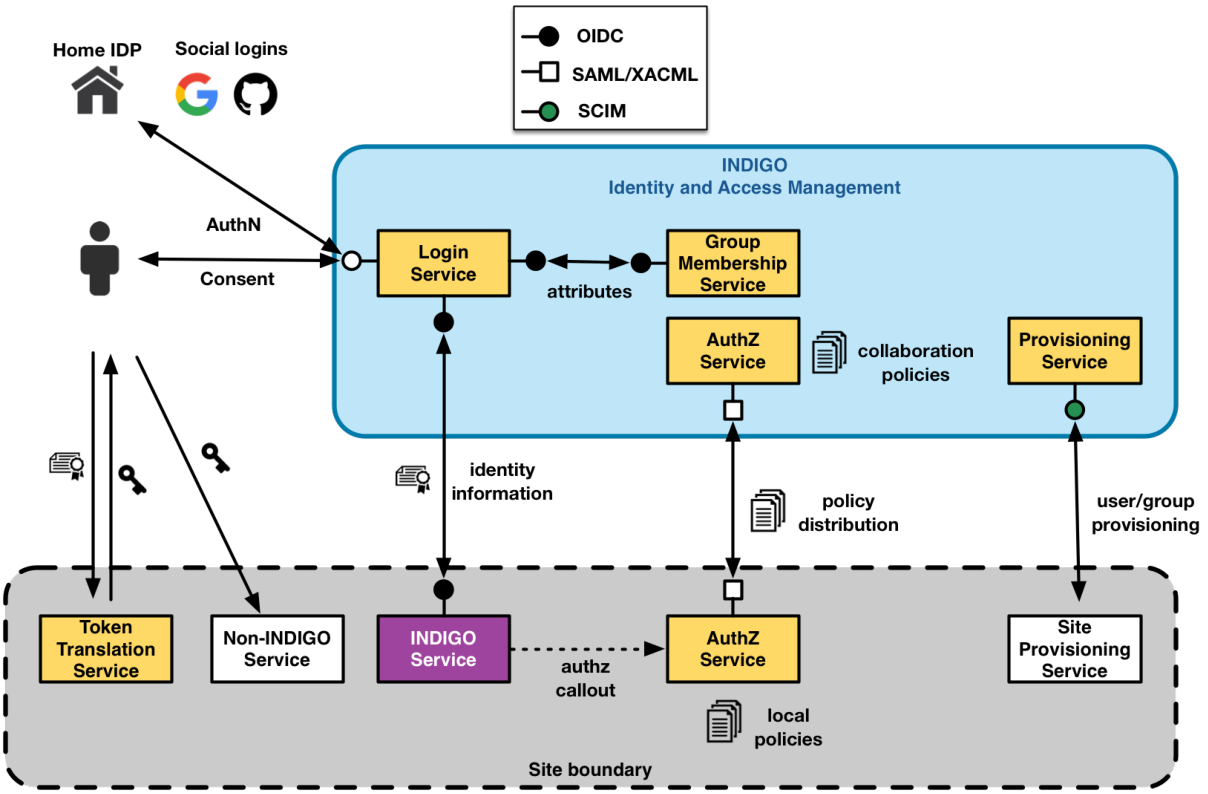
\includegraphics[width=10cm]{./figs/Figure0.pdf}
  \caption{Architecture of the INDIGO Identity and Access management Service}
  \label{fig:0}
\end{figure}


IAM is used internally to the PaaS layer in order to deal with the authorization of each user to the services, but also in order to deal with group membership and role management for each user. Users may present themselves with any of the three supported token types (X.509, OpenID Connect, SAML) and are able to access resources that support any of them. 

All the interaction across all the services will require an authentication based on a well-scoped token. The IAM service also provides the basic for building the Token Translation Service, WaTTS.  

{\bf WaTTS}\footnote{https://github.com/indigo-dc/tts} is the INDIGO Token Translation Service. WaTTS allows using any legacy service with federated identities, such as eduGain or Google. For this, WaTTS accepts federated identities (via OpenID Connect) and uses a plugin scheme to generate credentials for your service. This allows the provision of services that do not normally support federated identities to federated users.




\subsection{Virtual Networks}


The INDIGO PaaS layer has been developed to exploit a wide range of cloud management frameworks (e.g. OpenStack, OpenNebula, Google Compute Engine, Microsoft Azure, Amazon EC2) and combine resources provided by these frameworks to enable the deployment of complex distributed applications. Each cloud management framework may exhibit a different native API and often these APIs can be configured in different ways. This heterogeneity constitutes a challenge when transparent instantiation of cloud resources across multiple frameworks is required. 
The INDIGO PaaS layer supports both common native APIs as well as the {\bf Open Cloud Computing Interface}\footnote{http://occi-wg.org/} ({\tt OCCI}). The OCCI specification is a standard from the {\bf Open Grid Forum}\footnote{https://www.ogf.org} that provides a flexible and extensible API to access and manage cloud resources. Although OCCI provides a convenient uniform API, its support to manage the network environment is limited in what concerns the setup of public/private network accessibility. Depending on the actual cloud management framework being used the target cloud may need manual network configuration prior to the use of OCCI. To address these problems INDIGO has defined and implemented an OCCI network extension that allows the network environment to be properly setup via the OCCI API regardless of the underlying cloud management framework.

For OpenNebula\cite{OPENNEBULA} sites the solution consists in a {\bf Network Orchestrator Wrapper} (NOW) \footnote{https://github.com/indigo-dc/now} and a corresponding backend in the {\bf rOCCI-server}\footnote{https://github.com/the-rocci-project/rOCCI-server}. NOW enforces site-wide policy and network configuration by making sure that only LANs designated by site administrators are made available to users, and that users cannot reuse LANs assigned to others while they remain reserved. NOW has been released with INDIGO, and the backend has been provided as a contribution to upstream rOCCI-server distribution.

For OpenStack, the OpenStack OCCI Interface (OOI) has been extended with support for advanced networking functions provided by OpenStack’s Neutron component such as router, network and subnet setup. The contribution was accepted upstream and is distributed with the OOI implementation.

The networking features of the OCCI gateway for the Amazon’s EC2 API were adjusted making sure that the model of setting up and using local virtual networks is in accordance with the model used in the other cloud management frameworks.

In addition a Virtual Router was implemented allowing networks to span across cloud  sites,  potentially geographically  distant,  so  that  a custom  networking  environment  can  be  setup  even if the resources are allocated in different cloud sites. The virtual router is a virtual machine that can be started via OCCI and makes use of {\bf OpenVPN}\footnote{https://openvpn.net} to implement network tunnels. The Virtual Routers can be intantiated by the PaaS layer to orchestrate the interconnection of virtual machines across cloud providers.




%%% Giacinto new text %%%%%%%%%

\section{Architecture of the platform as a service}
\label{sec:paas}

Generally speaking, a Platform as a Service (PaaS) is a software suite, which is able to receive programmatic resource requests from end users, and execute these requests provisioning the resources on some e-infrastructures. We can see already many examples in the industrial sector, in which open source PaaS solutions (eg. OpenShift\cite{OPENSHIFT} or Cloudfoundry are being deployed to support the work of companies in different sectors.

The case of supporting scientific users is more complex in general than supporting commercial activities, because of the heterogeneous nature of the infrastructures at the IaaS level (i.e. the resource centers) and of the inherent complexity of the scientific work requirements. The key point is to find the right agreement to unify interfaces between the PaaS and IaaS levels.

In order to better adapt to the wide range of use cases provided by the users communities we decided to take a different approach from many of the more used PaaS: our solution is based on the concept of orchestrating complex cluster of service and on the possibility to automatize the actions needed to implement the use cases. 
This approach was really succesful as it gave the possibility to implement also legacy applications and did not depended by the languange in which the application is build. 
 

In Figure \ref{fig:2} we show the general interaction between the IaaS and PaaS layers. 



\begin{figure}
  \centering
  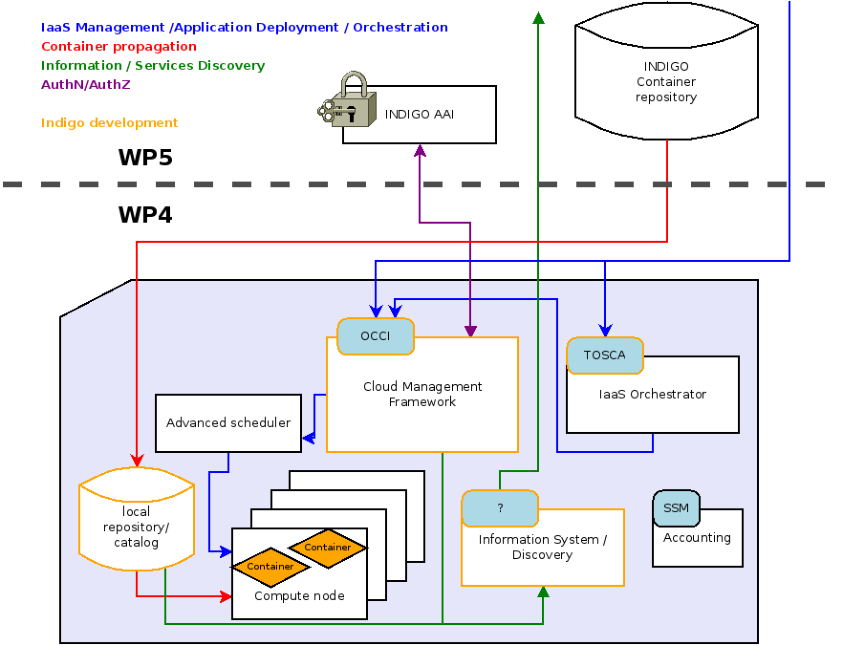
\includegraphics[width=\textwidth]{./figs/Figure2.pdf}
  \caption{Interaction between the IaaS and PaaS layers}
  \label{fig:2}
\end{figure}

INDIGO has provided a working PaaS Layer orchestrating heterogeneous computing and storage resources. Using PaaS Orchestrator together with the IM and TOSCA Templates, the end users are able to exploit computational resources without knowledge about the IaaS details. 

In the following we describe the main technologies employed to build the PaaS.  

\subsection{PaaS layer and microservices architecture}

The Paas layer should be able to hide complexity and federate resources for both Computing and Storage. For that we have applied the current technologies based on lightweight containers and related virtualization developments using on microservices. 

Kubernetes\cite{KUBERNETES}, an open source platform to orchestrate and manage Docker containers is  used to coordinate the microservices in the PaaS layer. Kubernetes is extremely useful for the monitoring and scaling of services, and to ensure their reliability. The PaaS manages the needed micro-services using Kubernetes, in order, for example, to select the right end-point for the deployment of applications or services.  The Kubernetes solution is used in the PaaS layer as is provided by the community. 

The microservices that compose the PaaS layer are very heterogeneous in terms of development: some of them are developed ad hoc, some others were already available and are used as they are, few others are deeply modified in order to implement new features within INDIGO. 

The language in which the INDIGO PaaS receives end user requests is TOSCA\cite{TOSCA}. TOSCA stands for Topology and Orchestration Specification for Cloud Applications. It is an OASIS specification for the interoperable description of application and infrastructure cloud services, the relationships between parts of these services, and their operational behaviour. 

TOSCA has been selected as the language for describing applications, due to the wide-ranging adoption of this standard, and since it can be used as the orchestration language for both OpenNebula (through the IM) and OpenStack (through Heat).

The released INDIGO PaaS layer (see Figure \ref{fig:3}) is able to provide automatic distribution of the application and/or services over a hybrid and heterogeneous set of IaaS infrastructures, on both private and public clouds. 



\begin{figure}
  \centering
  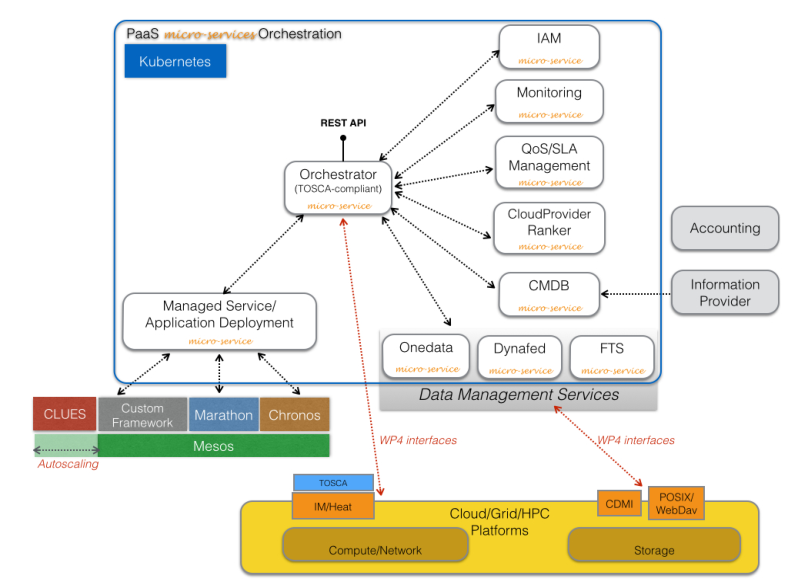
\includegraphics[width=\textwidth]{./figs/Figure3.pdf}
  \caption{Architecture of the INDIGO Platform as a Service layer.}
  \label{fig:3}
\end{figure}



The PaaS layer is able to accept a description of a complex set, or cluster, of services/applications by mean of TOSCA templates, and is able to provide the needed brokering features in order to find the best fitting resources. During this process, the PaaS layer is also able to evaluate data distribution, so that the resources requested by the users are chosen by the closeness to the storage services hosting the data requested by those specific applications/services.

\begin{figure}
  \centering
  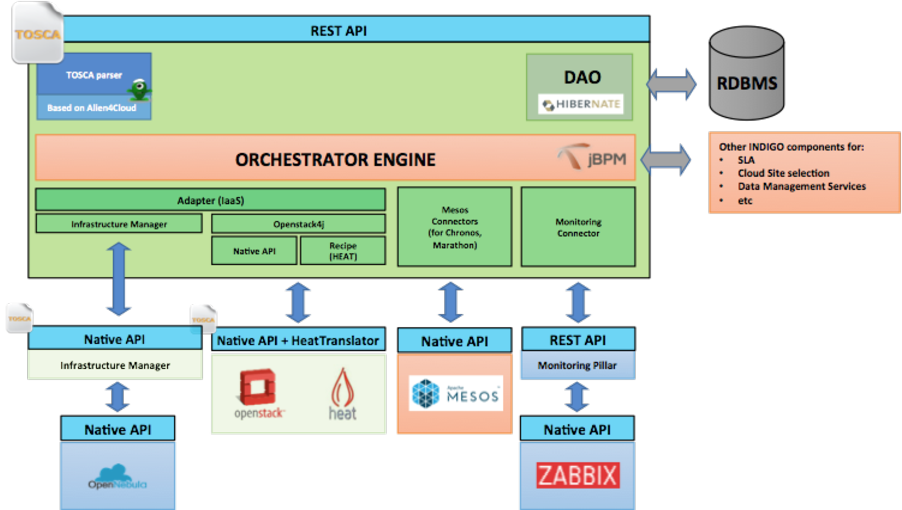
\includegraphics[width=\textwidth]{./figs/Figure4.pdf}
  \caption{Architecture of the Orchestrator within the PaaS layer.}
  \label{fig:4}
\end{figure}



\subsubsection{The Orchestrator Engine}


The INDIGO PaaS {\bf Orchestrator}\footnote{https://github.com/indigo-dc/orchestrator} is a component of the PaaS layer that allows to instantiate resources on Cloud Management Frameworks (like OpenStack and OpenNebula) and Mesos clusters.

It takes the deployment requests, expressed through templates written in TOSCA, and deploys them on the best cloud site available. In order to do that it gathers SLAs, monitoring info and other data from other platform services and it asks the {\bf Cloud Provider Ranker}\footnote{https://github.com/indigo-dc/cloudproviderranker} for a list of the best cloud sites. Therefore the Orchestrator mission is to coordinated the deployment process over the IaaS platforms. See Figure \ref{fig:4} for an overview of the orchestrator architecture.

The Orchestrator is based on developments already done in other publicly funded projects, as the Italian PONs PRISMA\cite{PRISMA}, and Open City Platform\cite{OPENCITY}. During the INDIGO project, this component has been extended and enhanced to support the specific microservices building the INDIGO PaaS Layer. It delegates the actual deployment of resources to IM, OpenStack Heat or Mesos frameworks based on TOSCA templates and the ranked list of sites.

A very innovative component is the Cloud Provider Ranker. This is a standalone REST web service, which ranks cloud providers on the basis of rules defined per user/group/use case, with the aim of fully decoupling the ranking logic from the business logic of the Orchestrator.

It allows the consumers of the service (one or more orchestrators) to specify preferences: if preferences have been specified, then they have absolute priority over any other provider information (like monitoring data); on the contrary, when preferences are not specified, for each provider the rank is calculated, by default, as the sum of SLA ranks and a combination of monitoring data, conveniently normalized with weights specified in the Ranker configuration file (with the last update the ranking algorithm can be customized to the specific needs).

This is a completely new service, fully implemented within the INDIGO project; it is based on an open source tool, Drools\footnote{https://www.drools.org}, in order to reduce the needed development effort, and to simplify the long-term support.

As a summary, one of the main achievements of INDIGO in this respect is the implementation of TOSCA Templates on IaaS that do not support natively TOSCA, like Standard OpenStack, OpenNebula, or Public clouds (like Microsoft Azure, AWS, OTC,...) using the Infrastructure Manager.

In particular, using the PaaS Orchestrator + IM + TOSCA Template the end user can exploit computational resources without knowledge about the IaaS details.


\subsubsection{High-level geographical applications/service deployment}

Using our {\bf CloudProviderRanker} the INDIGO PaaS is able to rank available resources given a defined set of rules (Reliability, Performance, etc). 

INDIGO has developed the tools and services to provide a solution for orchestrating Docker containers for both applications (job-like execution) and long running services, the {\bf MSA} service, which is based on top of {\bf Mesos/Marathon/Chronos}\footnote{https://github.com/indigo-dc/mesos-cluster}.

The MSA service provides full reliability  in case of failures, and scalability depending on the load on the specific services. It is also possible to describe  dependencies among the services in a complex cluster or in job-like execution  (the cluster and the jobs are described using TOSCA Templates).

It is also possible using the service {\bf CLUES}\footnote{https://github.com/indigo-dc/clues-indigo} (Cluster Energy Saving) to auto-scale (up \& down) depending on the load, on several types of clusters: Mesos, SLURM, PBS, HTCondor, etc. CLUES is an elasticity manager system for HPC clusters and Cloud infrastructures that features the ability to power on/deploy working nodes as needed (depending on the job workload of the cluster) and to power off/terminate them when they are no longer needed.

The submission of jobs uses an approach very similar to a batch system, exploiting resources where there are, without even knowing about the details. This includes deployment on multiple IaaS both private and public, hiding to the end users the complexity of the distributed resources.

The sustainability of our PaaS layer relies heavily on the fact that we have used Open Source frameworks where already available. 


\subsubsection{Data Management Services}

Data management services are based on three open source components: OneData\cite{ONEDATA}, DynaFed\cite{DYNAFED} and FTS3\cite{FTS}.

INDIGO has invested a substantial effort in the development of {\bf OneData}\footnote{https://github.com/indigo-dc/onedata}, this is a global data management system aiming to provide easy access to distributed storage resources. The finall goal is supporting a  wide  range  of  use  cases  from  personal  data  management  to  data-intensive  scientific  computations. 

The OneData development roadmap includes several data management related functionalities, among the most relevant ones:

\begin{itemize}
\item Cloud based data access
\item POSIX based data access
\item Data location
\item Data migration
\item Metadata management
\item ACL management
\item QoS and policy management
\end{itemize}

The OneData roadmap includes also adding features to support federated HPC applications, allowing transparent access to storage resources from multiple data centers simultaneously. OneData automatically detects whether data is available on 
local storage and can be accessed directly, or whether it has to be fetched from remote sites in real time. 

Support for federation in  OneData can be achieved by the possibility of establishing a distributed provider registry, where various infrastructures can setup their own provider registry and build trust relationship between these instances, allowing users from various platforms to share their data transparently.

OneData  provides  an  easy  to  use  Graphical  User  Interface  for  managing  storage  Spaces,  with customizable   access   control   rights   on   entire   data   sets   or   single   files   to   particular   users   or groups. 


%%%%%%%%%%%%%%%%%%%%%%%%%%%%%%%




\section{Interfacing with the users}
\label{sec:users}

Users typically do not access the PaaS core directly. They instead often use Graphical User Interfaces or simpler APIs. A user authenticated on the INDIGO Platform can access and customize a rich set of TOSCA-compliant templates through a GUI-based portlet.

The INDIGO repository provides a catalogue of pre-configured TOSCA templates to be used for the deployment of a wide range of applications and services, customizable with different requirements of scalability, reliability and performance. 

In those templates a user can choose between two different examples of generic scenarios:
 
\begin{enumerate}
\item Deploy a customized virtual infrastructure starting from a TOSCA template that has been imported, or built from scratch: The user will be able to access the deployed customized virtual infrastructure and run/administer/manage applications running on it.

\item Deploy a service/application whose lifecycle will be directly managed by the PaaS platform: in this case the user will be returned the list of endpoints to access the deployed services.
\end{enumerate}

INDIGO has provided the tools for a simple and effective end user experience, both for software developers and for researchers running the applications. 

APIs accessing the INDIGO PaaS layer are available, so that its features can be exploited by Portals, Desktop Applications and Mobile Apps. The final release of INDIGO-DataCloud software includes a large set of components to facilitate the development of Science Gateways and desktop/mobile applications, big data analytics and scientific workflows. 

In Figures \ref{fig:17} and \ref{fig:18} we show how to launch an application using a movil platform developed in the project. 


\begin{figure}
  \centering
  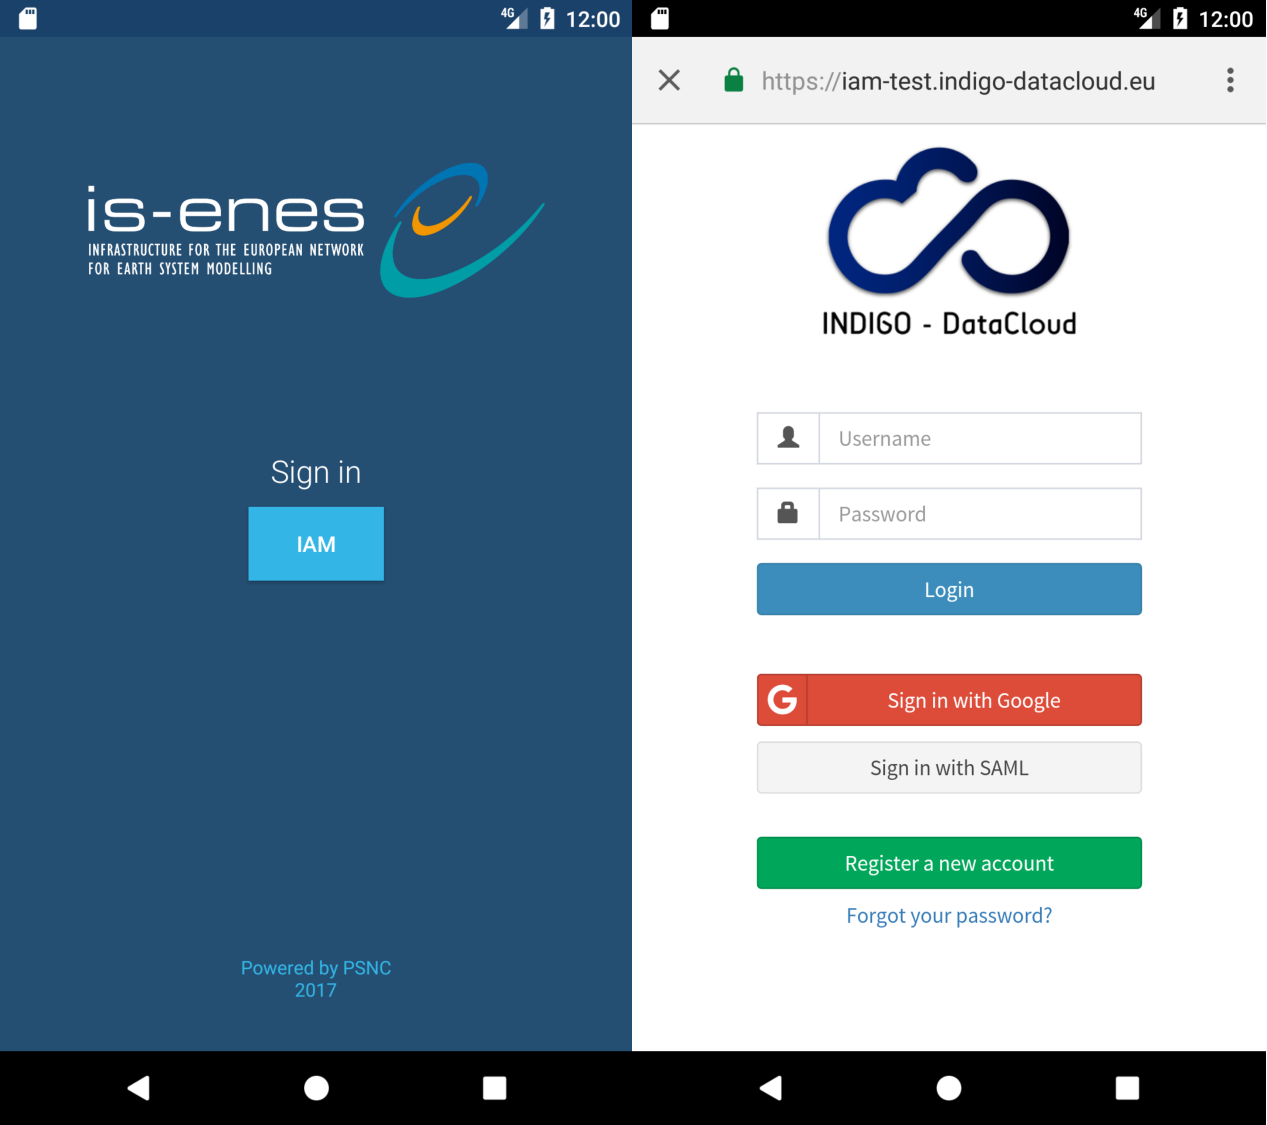
\includegraphics[width=\textwidth]{./figs/Figure17.pdf}
  \caption{Authentication of users on a mobile platform using IAM}
  \label{fig:17}
\end{figure}


\begin{figure}
  \centering
  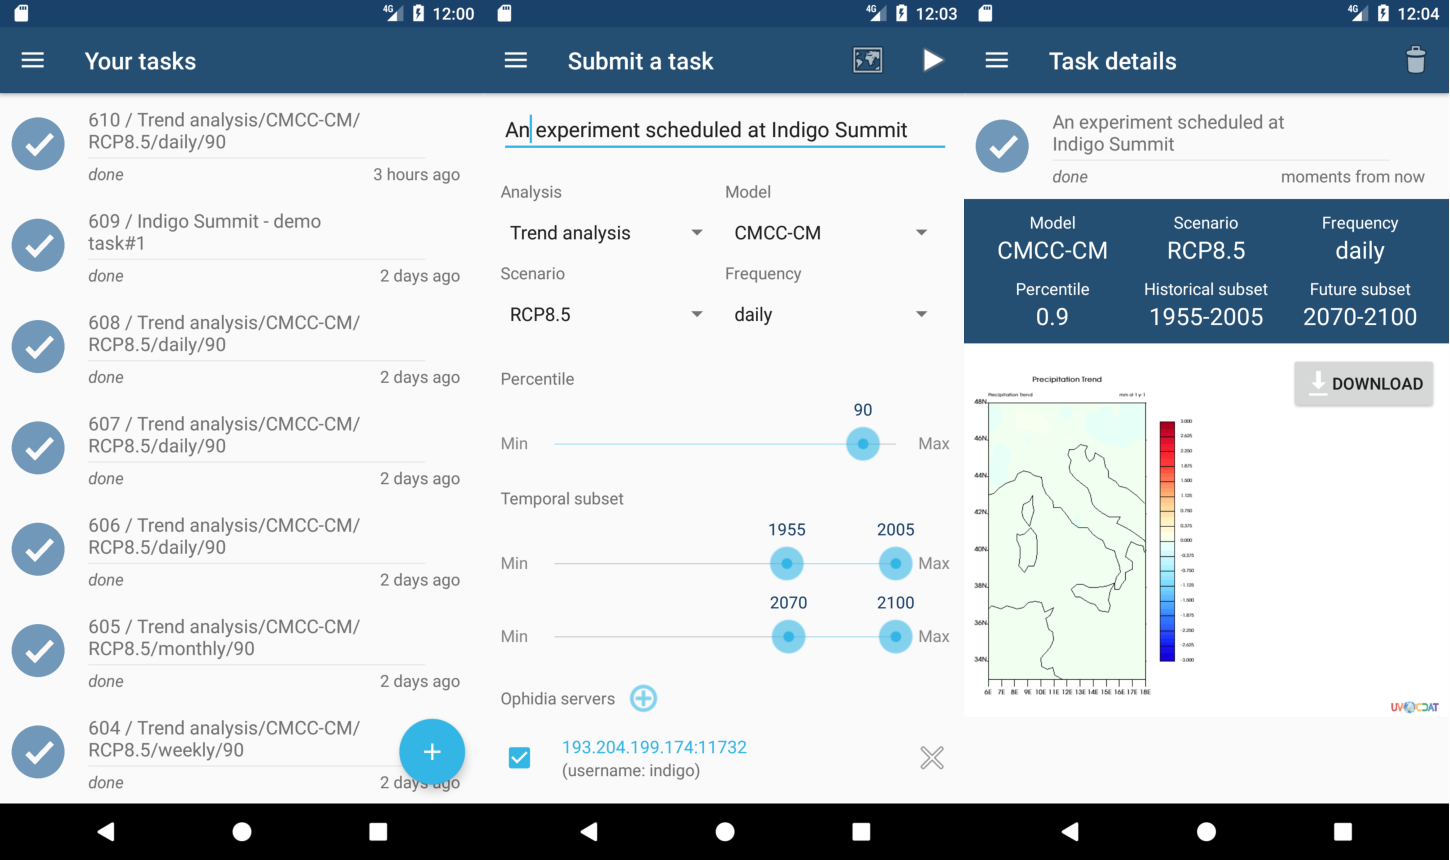
\includegraphics[width=\textwidth]{./figs/Figure18.pdf}
  \caption{Task submission and visualization of results on the mobile platform for ENES}
  \label{fig:18}
\end{figure}


In particular, components directly related to end user interfaces are: 

\begin{itemize}
\item The INDIGO FutureGateway (FG) framework, used to build powerful, customized, easy to use, science gateway environment and front-ends, on top of the INDIGO-DataCloud PaaS layer and integrated with data management services. The FG provides many capabilities, including: 
\item The FG API server, used to integrate third-party science gateways; the FG Liferay Portal, containing base portlets for the authentication, authorization and administration of running applications and deployments; 
\item Customizable Application Portlets, for user-friendly specification of the parameters used by TOSCA templates;  
\item A workflows monitoring portlet, used for monitoring task execution via integrated workflow systems, described below. 
\item An Open Mobile Toolkit as well as application templates for Android and iOS, simplifying the creation of mobile apps making use of the FG API Server. 
\item Support for scientific workflows, where the INDIGO components: 
\begin{itemize}
\item Provide dynamic scalable services in a Workflows as a Service model;
\item Implement modules and components enabling the usage of the PaaS layer (via FG API Server) for the main scientific workflow engines deployed by user communities (such as Kepler, Ophidia, Taverna,Pegasus);  
\item Support a two-level (coarse and fine grained) workflow orchestration, essential for complex, distributed experiments involving (among others) parallel data analysis tasks on large volumes of scientific data.    
\end{itemize}
\item Key extensions to the Ophidia big data analytics framework (allowing to process, transform and manipulate array-based data in scientific contexts), providing many new functionalities, including a set of new operators related to data import regarding heterogeneous data formats (e.g. SAC, FITS), a new OpenIDConnect interface and new workflow interface extensions. 

\item Enhancements of the jSAGA library through a "Resource Management API", complementing the standard Job/Data Management API. This allows to acquire and manage resources (compute, storage, network) and enables the wrapping of underlying technologies (cloud, pilot jobs, grid, etc.) by means of a single API, supporting asynchronous mode (task), timeout management, notification (metrics) and security context forwarding. 

\item Command-line clients for the PaaS layer to provide an easy way for users to interact with the Orchestrator or with WATTS:
\begin{itemize}
\item {\bf Orchent}\footnote{https://github.com/indigo-dc/orchent}: a command-line application to manage deployments and their resources on the INDIGO-DataCloud Orchestrator;
\item {\bf Wattson}\footnote{https://github.com/indigo-dc/wattson}: a command-line client for the INDIGO Token Translation Service.
\end{itemize}

\end{itemize}



%% New section 6 %%%%%%%%%%%%


\section{Software lifecycle management and release process}
\label{sec:release}

The software lifecycle process in INDIGO has
been supported by a continuous software improvement process that
encompasses software quality assurance, software
release and maintenance, support services, and the pilot infrastructures needed
for software integration and testing.

Following the successful examples of other research software
development projects like, EGEE I, II, III, and EMI, the development,
maintenance and evolution of the software is taken over by the Product Teams (PTs). PTs are small teams of software developers, fully responsible for the development of a particular software product (or group of tightly related products) compliant with the project's acceptance criteria.

\begin{figure}
  \centering
  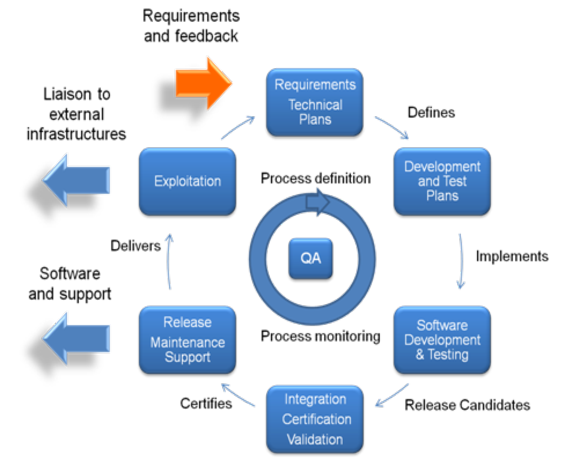
\includegraphics[width=\textwidth]{./figs/Figure5.pdf}
  \caption{Software lifecycle implementation}
  \label{fig:5}
\end{figure}


Preview releases are made available for evaluation by user communities and
resource providers through the pilot infrastructures. Release
candidates are subjected to integration testing, which may include the
participation of user communities. Once the required release quality is
attained the software is made available to the general public through
INDIGO-DataCloud repositories. INDIGO then provides support for the released
software and manage bug fixes in close coordination with the developers.


\subsection{Software development process}


Software Quality Assurance (SQA) is performed mostly via
automated actions orchestrated by a tool. Each change in the source code,
meant to be integrated in the production version, triggers the associated
quality control checks, defined as jobs in the CI system. These jobs
themselves are defined by the PTs together with the quality assurance and
release teams, covering code style checking,
unit testing, functional testing and, whenever possible, integration testing.
Some manual steps, e.g. for documentation verification and code review, are
also required. The requirements were defined early in the
project lifetime and have evolved into a consolidated document to be
used in a more broader context \cite{SQA}.

In Figure \ref{fig:6} we depict the project's software
lifecycle workflow showcasing the interdependencies between
the quality control, release, maintenance and exploitation activities, together
with the services involved at each stage. Figure \ref{fig:7} highlights the set of tools and services needed to support the software development process.


\begin{figure}
  \centering
  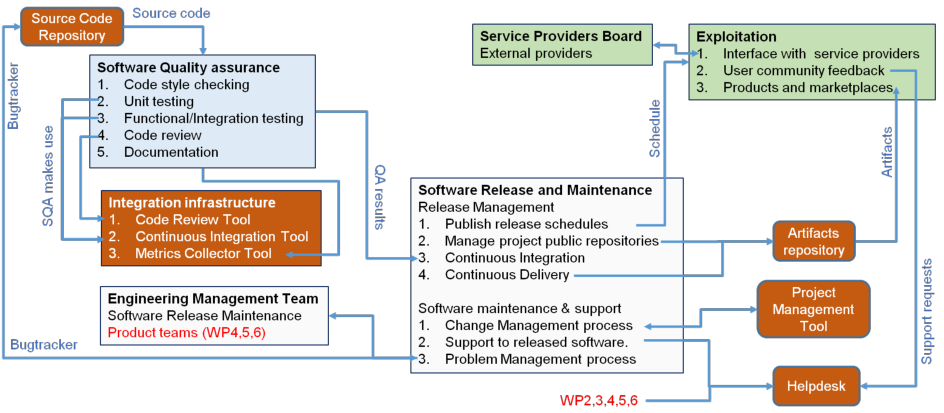
\includegraphics[width=\textwidth]{./figs/Figure6.pdf}
  \caption{Software lifecycle, release, maintenance and exploitation interdependencies.}
  \label{fig:6}
\end{figure}



\begin{figure}
  \centering
  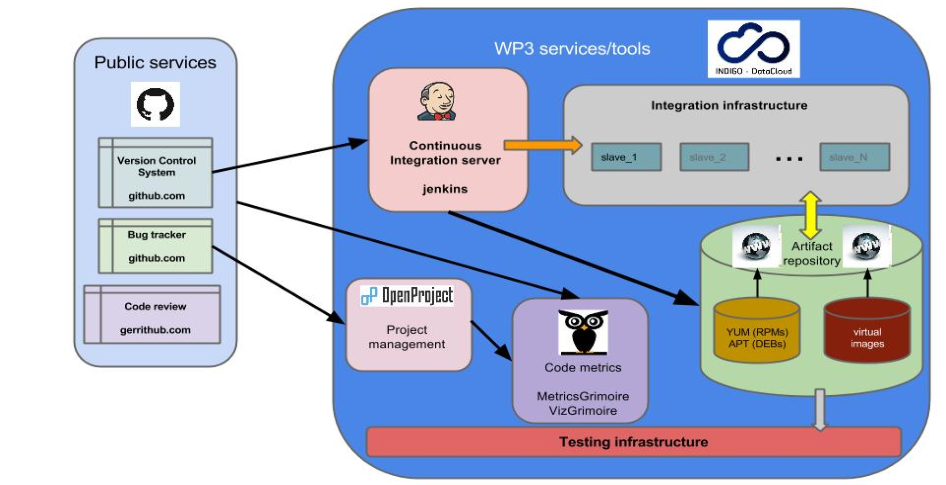
\includegraphics[width=\textwidth]{./figs/Figure7.pdf}
  \caption{Tools and services used to support the software development Product Teams.}
  \label{fig:7}
\end{figure}


\begin{itemize}
    \item Project management service using {\bf openproject.org}: It provides
        tools such as an issue tracker, wiki, a placeholder for documents and a
        project management timeline.

    \item Source code is publicly available, housed externally
        in GitHub repositories, increasing so the visibility and simplifying the path to exploitation beyond the project lifetime. The INDIGO-DataCloud software is released under the Apache 2.0 software license \cite{apache-license}.

    \item Continuous Integration service using {\bf Jenkins}: Service to
        automate the building, testing and packaging, where
        applicable. Testing includes the style compliance and
        estimation of the unit and functional
        test coverage of the software components.

    \item Artifact repositories for RedHat and Debian
        packages \cite{indigo-package-repo} and virtual -- Docker -- images
        \cite{indigo-dockerhub}.

    \item Code review service using GitHub: Source code
        review is one integral part of the SQA
        as it appears as the last step in the change
        verification process. This service facilitates the code review
        process, recording the comments and
        allowing the reviewer to verify the candidate change before
        being merged into the production version.

    \item Issue tracking
        using GitHub Issues: Service to track issues, new features and bugs of
        INDIGO-DataCloud software components.

    \item Release notes, installation and configuration guides, user and
        development manuals are made available on {\bf GitBook}
        \cite{indigo-gitbook}.

    \item Code metrics services using {\bf Grimoire}: To collect and visualize
        several metrics about the software components.

    \item Integration infrastructure: this infrastructure is composed of
        computing resources to support directly the CI service.

    \item Testing infrastructure: this infrastructure aims to provide
        a stable
        environment for users where they can preview the software and services
        developed by INDIGO-DataCloud, prior to its public release.

    \item Preview infrastructure: where the released artifacts are deployed and
        made available for testing and validation by the use-cases.
\end{itemize}



\subsection{DevOps approach in INDIGO}

Progressive levels of automation were being adopted throughout
the different phases of the INDIGO-DataCloud project software development and
delivery processes. This evolution was intentionally marked by the commitment
to DevOps principles \cite{devops}. Starting with a continuous integration
approach, achieved already in the early stages of the project, the second part
of the project was devoted to the establishment of the next natural step in the
DevOps practices: the continuous delivery (CD).

\subsubsection{Services for continuous integration and SQA}

The INDIGO-DataCloud CI process is schematically shown
in Figure \ref{fig:8}. The process, in its different steps, reflects some of
the main and important achievements of the software integration team, such as:

\begin{figure}
  \centering
  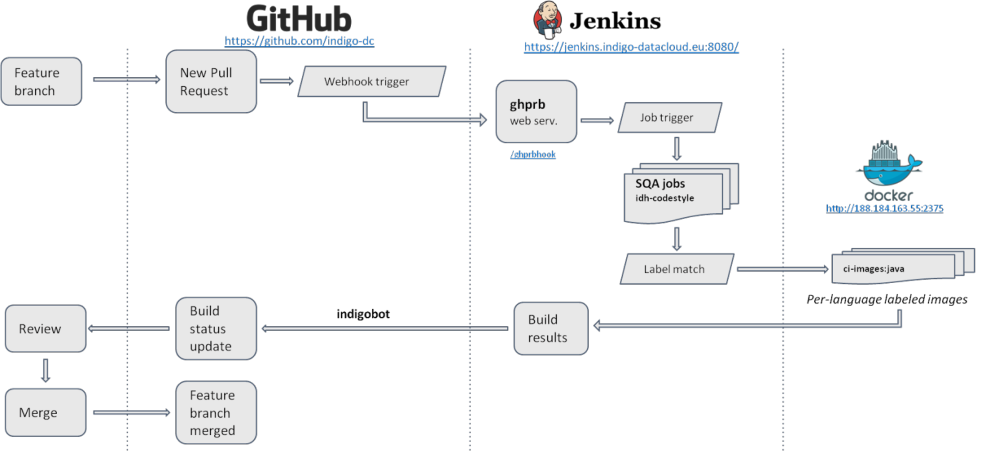
\includegraphics[width=\textwidth]{./figs/Figure8.pdf}
  \caption{Continuous Integration workflow followed by new feature additions in the production codebase.}
  \label{fig:8}
\end{figure}

\begin{itemize}
    \item New features are developed independently from the
          production version in \textit{feature branches}. The creation of
          a pull request for a specific feature branch marks the start of
          the automated validation process through the execution of the
          SQA jobs.

    \item The SQA jobs perform the code style verification and calculate unit
        and functional test coverage.
        \begin{itemize}
            \item The tools necessary for tackling these tests are packaged in
                Docker images, available in DockerHub.
            \item Each test then initiates a new container that provides a
                clean environment for its execution.
            \item This is an innovative approach that provides the flexibility
                needed to cope with the INDIGO-DataCloud software diversity.
        \end{itemize}

    \item The results of the several SQA jobs are made available in the Jenkins
        service which notifies back to GitHub their exit status.
        \begin{itemize}
            \item Only if the tests have succeeded, the source code is
                validated and is ready to be merged into the production branch.
        \end{itemize}

    \item The last step in the workflow is the code review, where a human
        review of the change is performed. After code review the source code
        can be merged and becomes ready for integration and later release.
\end{itemize}



As a general rule, the described CI process must be followed by all the PTs
contributing code to INDIGO-DataCloud. However there are exceptions to this rule that fall into two main categories:

\begin{itemize}
    \item mature products that have well established development services
        already in place;

    \item new software products that aim to contribute to existing
        projects/frameworks (such as OpenStack, OpenNebula and
        others), which make use of dedicated
        development services made available by the corresponding projects.
\end{itemize}

For these cases where products are using external development services, the
PTs must account that:
\begin{itemize}
    \item CI testing must satisfy the INDIGO-DataCloud SQA requirements;

    \item Provisioning of metrics could be requested by the SQA
        team.

\end{itemize}

The INDIGO-DataCloud SQA team keeps track of the exceptions and continuous
integration systems being used by the several products. This is a dynamic
process. As products evolve and become accepted in their target projects they
may move from the INDIGO-DataCloud development system to external development
systems.

This is indeed one of the objectives of the SQA in INDIGO-DataCloud, improve
the quality of the software, so that it can be more easily accepted in target
projects ensuring a path for sustainability and exploitation.

\subsubsection{Continuous delivery}
Continuous delivery adds, on top of the software development chain, a seamless
manufacturing of software packages ready to be deployed into production
services. Therefore, fast, frequent and small releases can be taken over thus
promoting the reliability of the software.

In the INDIGO-DataCloud scenario, the continuous delivery adoption translates
into the definition of pipelines. A pipeline is a serial execution of tasks
that encompasses in the first place the SQA jobs (CI phase) and adds as the
second part (CD phase) the building and deployment testing of the software
packages created. The pipeline only succeeds if each task is run to completion,
otherwise the process is stopped and set as a build failure.

As a result, in one pipeline execution, the source code is validated and
packaged automatically, with the only manual intervention of approving and
marking the resulting packages as production-ready. As shown in Figure
\ref{fig:15}, these software pipelines where defined in the Jenkins CI service
and differ in the number of tasks depending on the packaging type being
produced: tarballs, RPM/DEB packages and/or Docker images.



\begin{figure}
  \centering
  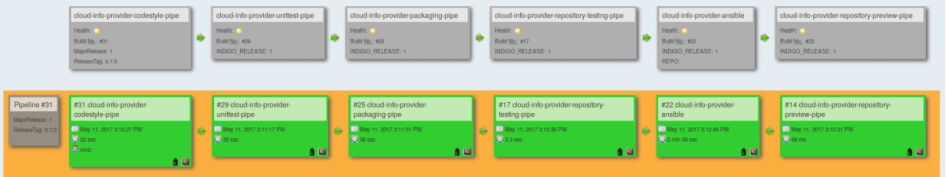
\includegraphics[width=\textwidth]{./figs/Figure15.pdf}
  \caption{DevOps pipeline to distribute Ubuntu Xenial and CentOS7 packages for cloud-info-provider product}
  \label{fig:15}
\end{figure}

\subsubsection{DevOps adoption from user communities}

The experience gathered throughout the project with regards to the adoption of
different DevOps practices is not only useful and suitable for the software
related to the core services in the INDIGO-DataCloud solution, but also
applicable to the development and distribution of the applications coming from
the user communities.

As an example, two applications DisVis and PowerFit, were integrated into a
similar CI/CD pipeline described above. As it can be seen in the Figure
\ref{fig:15}, with this pipeline in place the application developers were
provided with both a means to validate the source code before merging and the
creation of a new versioned Docker image, automatically available in the
INDIGO-DataCloud’s catalogue for applications i.e. DockerHub’s {\tt
indigodatacloudapps} repository.

The novelty introduced in the pipeline above is the validation of the user
application. Once the application is deployed as a Docker container, and
subsequently uploaded to {\tt indigodatacloudapps} repository, it is
instantiated in a new container to be validated. The application is then
executed and the results compared with a set of reference outputs. Thus this
pipeline implementation goes a step forward by testing the application
execution for the last available Docker image in the catalogue.

\begin{figure}
  \centering
  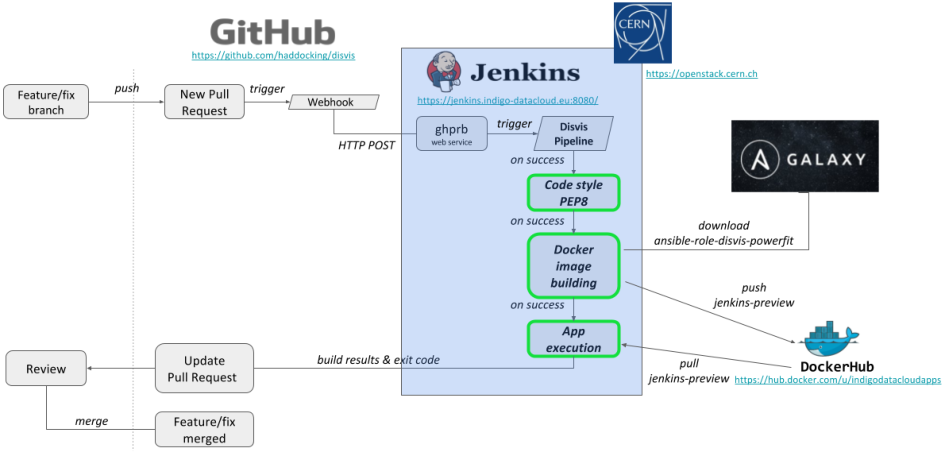
\includegraphics[width=\textwidth]{./figs/Figure16.pdf}
  \caption{DisVis development workflow using a CI/CD approach}
  \label{fig:16}
\end{figure}



\subsection{INDIGO-1 release ({\tt MidnightBlue})}

The first INDIGO-DataCloud major release - INDIGO-1 (codename {\tt MidnightBlue}) was released 1st of August 2016. The public availability was announced through:

\begin{itemize}
\item General announcements
\item On the project News:

https://www.indigo-datacloud.eu/news/first-indigo-datacloud-software-release-out
\item INDIGO-DataCloud RSS Feed:\\
http://repo.indigo-datacloud.eu/INDIGODataCloudNews.rss.xml
\item indigo-all mailing-list:\\
https://lists.indigo-datacloud.eu/sympa/arc/indigo-all/2016-08/msg00000.html
\end{itemize}

In table \ref{tab:1} we show the INDIGO-1 fact sheet.

\begin{figure}
  \centering
  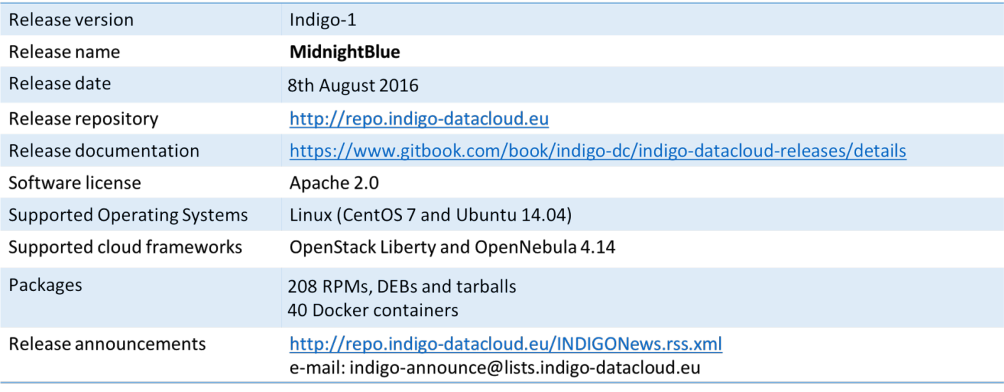
\includegraphics[width=\textwidth]{./figs/TableI.pdf}
  \caption{INDIGO-1 release fact sheet}
  \label{tab:1}
\end{figure}

\subsubsection{Contributions to Upstream Distribution}

Many of the INDIGO-DataCloud solutions released through INDIGO-1 were also contributed to the respective upstream distributions like:

\begin{itemize}
\item OpenStack
\begin{itemize}
\item Changes/contribution done already merged upstream
\begin{itemize}
\item Nova Docker
\item Heat Translator (INDIGO-DataCloud is 3rd overall contributor and core developer)
\item TOSCA parser (INDIGO-DataCloud is 2nd overall contributor and core developer)
\item OpenID Connect CLI support
\item OOI: OCCI implementation for OpenStack
\end{itemize}
\item Changes/contribution under discussion to be merged upstream
OpenStack Preemptible Instances support (extensions)
\end{itemize}
\item OpenNebula
\begin{itemize}
\item Changes/contribution done already merged upstream
\begin{itemize}
\item ONEDock
\end{itemize}
\end{itemize}
\item Changes/contribution done already merged upstream for:
\begin{itemize}
\item Infrastructure Manager
\item CLUES
\item OneData
\item jSAGA Adaptors
\item MitreID connect library
\end{itemize}
\end{itemize}


\subsection{INDIGO-2 release ({\tt ElectricIndigo})}

The second INDIGO-DataCloud major release - INDIGO-2 (codename {\tt ElectricIndigo}) was made publicly available on April 14th  2017. The release was announced through:
\begin{itemize}
\item General announcements
\begin{itemize}
\item On the project news: \\
https://www.indigo-datacloud.eu/news/electricindigo-second-indigo-datacloud-software-release
\end{itemize}
\item INDIGO-DataCloud RSS Feed: \\
http://repo.indigo-datacloud.eu/INDIGODataCloudNews.rss.xml
\end{itemize}

In table \ref{tab:2} we show the INDIGO-2 release fact sheet.

\begin{figure}
  \centering
  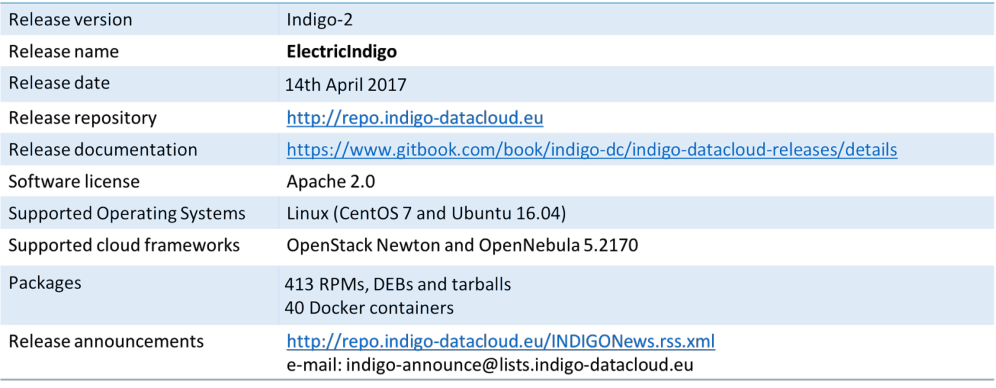
\includegraphics[width=\textwidth]{./figs/TableII.pdf}
  \caption{INDIGO-2 release fact sheet}
  \label{tab:2}
\end{figure}

\subsection{Software Stage Rollout}

The INDIGO-DataCloud Staged Rollout is a procedure based on EGI\cite{EGI} Staged Rollout whereby releases of the supported middleware are first deployed and tested by Service Providers who have agreed to be Early Adopter before being widely
disseminated to all Service Providers.

This procedure permits testing the artifacts in a production environment and exposing  the software to real endusers.

This environment is also more heterogeneous than what is possible during the certification and verification phases. The procedure  allows for potential issues to be discovered and workarounds to be swiftly added.

The Staged rollout takes place after the products are made available in the INDIGO-DataCloud repositories and constitute a last step of verification before the products are incorporated in other distributions such as EGI CMS and UMD. Users and site administrators unrelated to INDIGO-DataCloud can participate in the process.

\subsection{Software maintenance strategy and updates}

The software maintenance activity focus on the timely release of corrective (bug fixes) and adaptive (new/versions of operating systems and/or cloud management frameworks) changes as well as perfective and preventive ones, following the defined procedures.

The software support activities concentrate on following closely the different user communities and e-infrastructure sites that use and deploy projects solutions, ensuring that all their requests for support, for changes/improvements are addressed and correctly redirected to the right development teams, in case proven to be bugs in the released software.

Let us see with an example how the maintenance process of INDIGO-1 has smoothly worked out towards the release of INDIGO-2. Updates continued to be provided on a monthly manner taking in consideration that:

\begin{itemize}
\item After the release of the first INDIGO major release, MidgnightBlue, on August 2016, from the point of view of the schedule the activity entered in the Full Support period, period in which the developers were supposed to fix all the notified issues, according to their priority, and also to add missing or new features and improvements.
\item The full support period ended February 2017, so that no new features were added to INDIGO-1, but moved, eventually to INDIGO-2 release. During this Standard Support period the developers were due to release only bug fixes.
\item The Standard Support period ended at the end of March 2017, in concomitance with the release of  the projects’ second major release. No more changes, bug fixes were introduced. Just support for fixing security vulnerabilities for 2 more months, until the end of May 2017.
\item After May 2017 - INDIGO-1 repositories are closed, and the only supported components will be the ones present in the INDIGO-2 release. And so the MidnightBlue release reached the EndOfLife.
\end{itemize}


\begin{figure}
  \centering
  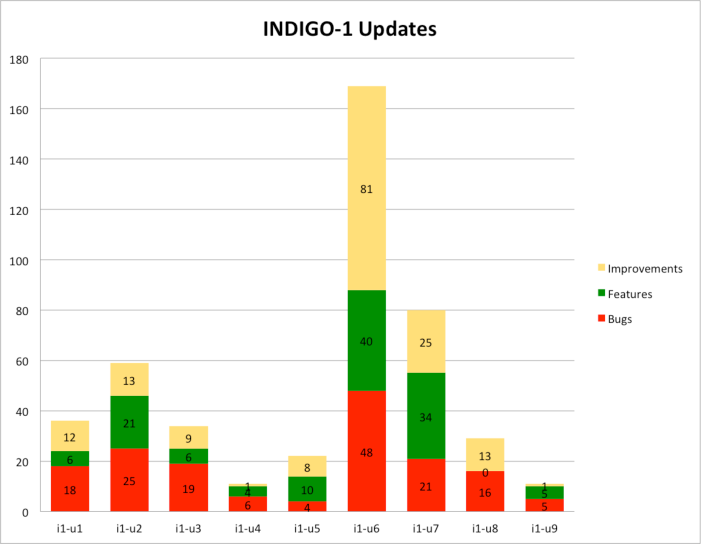
\includegraphics[width=\textwidth]{./figs/Figure9.pdf}
  \caption{Updates and maintenance of INDIGO-1 ({\tt MidnightBlue})}
  \label{fig:9}
\end{figure}


\begin{figure}
  \centering
  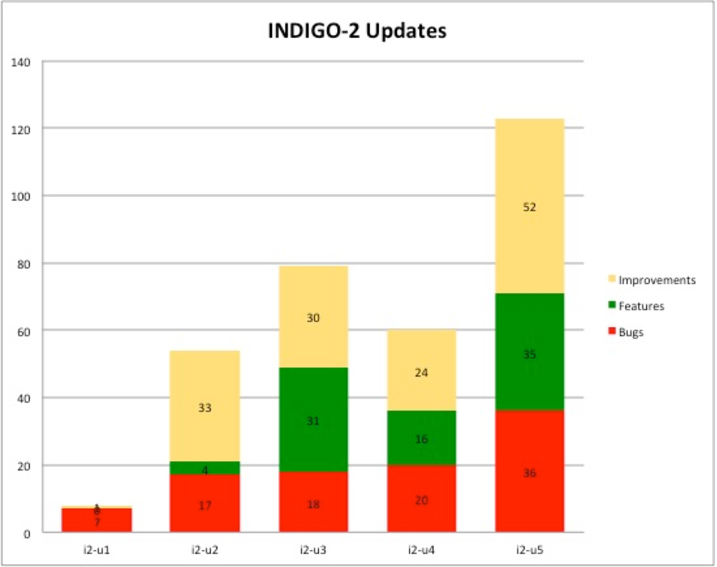
\includegraphics[width=\textwidth]{./figs/Figure10.pdf}
  \caption{Updates and maintenance of INDIGO-2 ({\tt ElectricIndigo})}
  \label{fig:10}
\end{figure}



During the full support period PTs managed to fix $\sim$ 98 issues and to add $\sim$ 226 new features \& improvements to the released services \& components, as detailed in Figures \ref{fig:9} and {\ref{fig:10}.

The above statistics are based on the information provided by the Product Teams in the release notes of each updated service or component. To conclude, we present in Table \ref{tab:3} the updated timelines of the INDIGO - Datacloud Maintenance and Support activities.


\begin{figure}
  \centering
  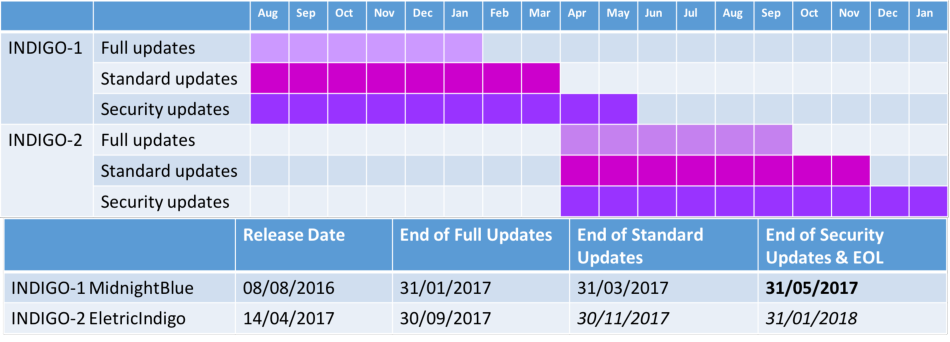
\includegraphics[width=\textwidth]{./figs/TableIII.pdf}
  \caption{Support timeline for the INDIGO releases}
  \label{tab:3}
\end{figure}



%%%%%%%%%%%%%%%%%%%%%%%%%%%%%%%%%


\section{Examples of implementation of results towards research communities}
\label{sec:examples}

In what follows we try to provide some basic information that may be useful for promoting the use of INDIGO solutions towards the Research Communities.

Based on the described architecture we will introduce the basic ideas on how to develop, deploy and support applications in the Cloud framework, exploiting the different service layers, and introducing generic examples that may make easier the use of INDIGO solutions.   



\subsection{Understanding services in the Cloud Computing framework}

Figure \ref{fig:11} provides the description of how an application can be built using a service oriented architecture in the Cloud, using INDIGO solutions. 

This layered scheme includes different elements, that are managed by different actors, that must be minimally understood in order to design, develop, test, deploy and put in production an application.

The lowest layer, Infrastructure as a Service, provides a way to access to the basic resources that the application will use, like computing, storage, network, etc. These resources are physically in a “site”, typically a computing center, either in a research centre, or in a “cloud provider” (like for example commercial cloud services), and are handled by the system managers at those sites, that install a IaaS solution compatible with the INDIGO software stack (e.g. OpenStack, OpenNebula, Google Compute Engine, Microsoft Azure, Amazon EC2). 

Accessing through a web interface to a proprietary dashboard, like for example Horizon for OpenStack, a “user” that is granted access to a pool of resources at a site (for example 150 cores in “virtual” machines with 600GB RAM, 3 TB of storage and 1GB network interface) can “launch” a virtual machine, for example a server with 2 cores, 4GB RAM, 100GB of storage and with a certain Linux flavour installed. 

The user can then get access in “console” mode to this machine, for example through a protocol like ssh, and employ it for the tasks required. For example, he can execute a simple script, or can install a web server, etc. When the work is finished the machine can be stopped by the user, liberating so the resources. This is a very basic mode of accessing Cloud services, which shares analogies with the usual access to classical computing services, like for example any remote server or a cluster.

A different way to interact with IaaS services is to use the existing APIs to manage the resources using the web services protocol. Such invocation of services can be made from any program or application, from example from a python script, and even through a web interface. 

Many applications require the setup, launching and interconnection of several (IaaS) services implemented in different virtual machines, and managed under a single control, as a “Platform”. The Platform as a Service (PaaS) layer enables this “orchestration” of IaaS services, and in the case of a “Federated Cloud” they might even be located in different sites. 


\begin{figure}
  \centering
  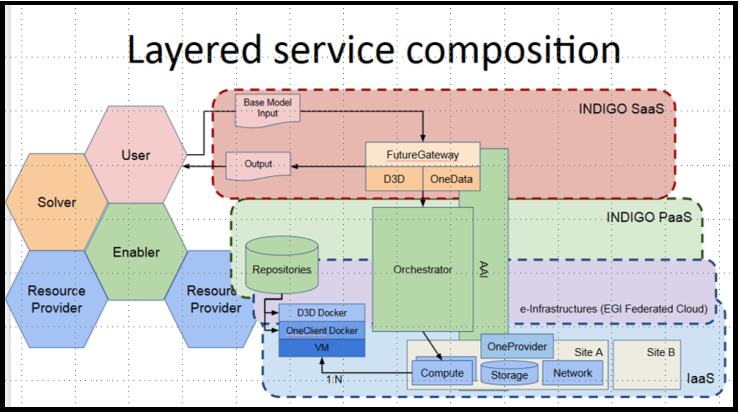
\includegraphics[width=\textwidth]{./figs/Figure11.pdf}
  \caption{Service composition in the Service Oriented Architecture}
  \label{fig:11}
\end{figure}


For example, an Apache Web may be launched in site 1, and display the output of a simulation running in a cluster launched on demand in site 2. The Apache Web service may be better supported with a pool of resources using another cloud-oriented solution like Marathon/Mesos.   Launching an application in this context is a non-trivial process, that requires identifying the available resources and launching them via the IaaS services. INDIGO is supporting the TOSCA standard to prepare a template that can be used to automatize this selection and orchestration of services.

However, most researchers are mainly interested in “running” a final application, either accessing it as an existing service, or eventually requesting resources and launching the application themselves, to use it afterwards. This possibility is enabled via the Software as a Service (SaaS) layer.

Before continuing to provide different examples and templates based on the previous discussion, we need a few words on the organization from the point of view of the research community.

\subsection{Building and executing applications using INDIGO solutions}


In what follows we present below several simple examples of basic, but generic, applications exploiting INDIGO solutions. 

\begin{itemize}

\item The first generic example is how to build an application encapsulated as a container and how to executed it in an HPC system.

This basic example of using INDIGO solutions is shown in Figure \ref{fig:13}. A user can create a container using a conventional Dockerfile which describes the steps required to create the Docker image. The process can be fully automatized using GitHub and Docker Hub in such a way that a change in the Dockerfile, immediately triggers a rebuilt of the application container.

INDIGO provides the udocker tool to enable execution of application containers in batch systems. The end-user can download the udocker Python script from GitHub or can send it with the batch job. Once executed for the first time it setups itself in the user home directory. udocker provides a Docker like command line interface with which the user can pull, import or load Docker containers and then execute them using a chroot-like environment. The software within the container must not require privileges during execution as it will be executed under the user that invokes udocker.


This is also a good solution for research communities that want to migrate towards a cloud-based framework using containers, but keep exploiting resources like grid-enabled clusters or even supercomputers. 

udocker is used by the Case Studies on Structural Biology (Powerfit and Disvis) exploiting grid resources, on Phenomenology in Particle Physics, and recently for Lattice QCD on supercomputers. Also, the TRUFA genomic pipeline exploits this solution, and it is being extended to similar applications in the area that require the integration of legacy libraries. 


\item The second example is how to build an application encapsulated as a container and launch it in the Cloud, from a web interface, using the INDIGO solutions FutureGateway and PaaS Orchestrator

This second example, compared to the first one, shows the evolution required to move an application to the Cloud arena: the application must be encapsulated into a container, as before, but to launch this container the cloud resources must be allocated, the user must authenticate and get the access granted. If different services are required, they must be orchestrated.


The way to express these requirements, using an open standard, is a TOSCA template. FutureGateway offers a user-friendly web-based interface to customize the TOSCA template, authenticate the user, select the container to be executed, interact with the Orchestrator to allocate the required cloud resources and launch the application. 

Like in the first example the container can be created using a dockerfile whose automation can be accomplished by using GitHub and Docker Hub.


Using the Future Gateway portal or the command line tool Orchent, the user can submit a TOSCA template to the Orchestrator, which in turn will request and allocate the resources at the IaaS level by asking the Infrastructure Manager to do so.

The user may wish to connect to the container that has been launched via the orchestrator using the {\tt ssh} command. Once in the container it is posible to mount remote data repositories or stage the output data using ONEDATA, available at the IaaS layer.

\end{itemize}


\begin{figure}
  \centering
  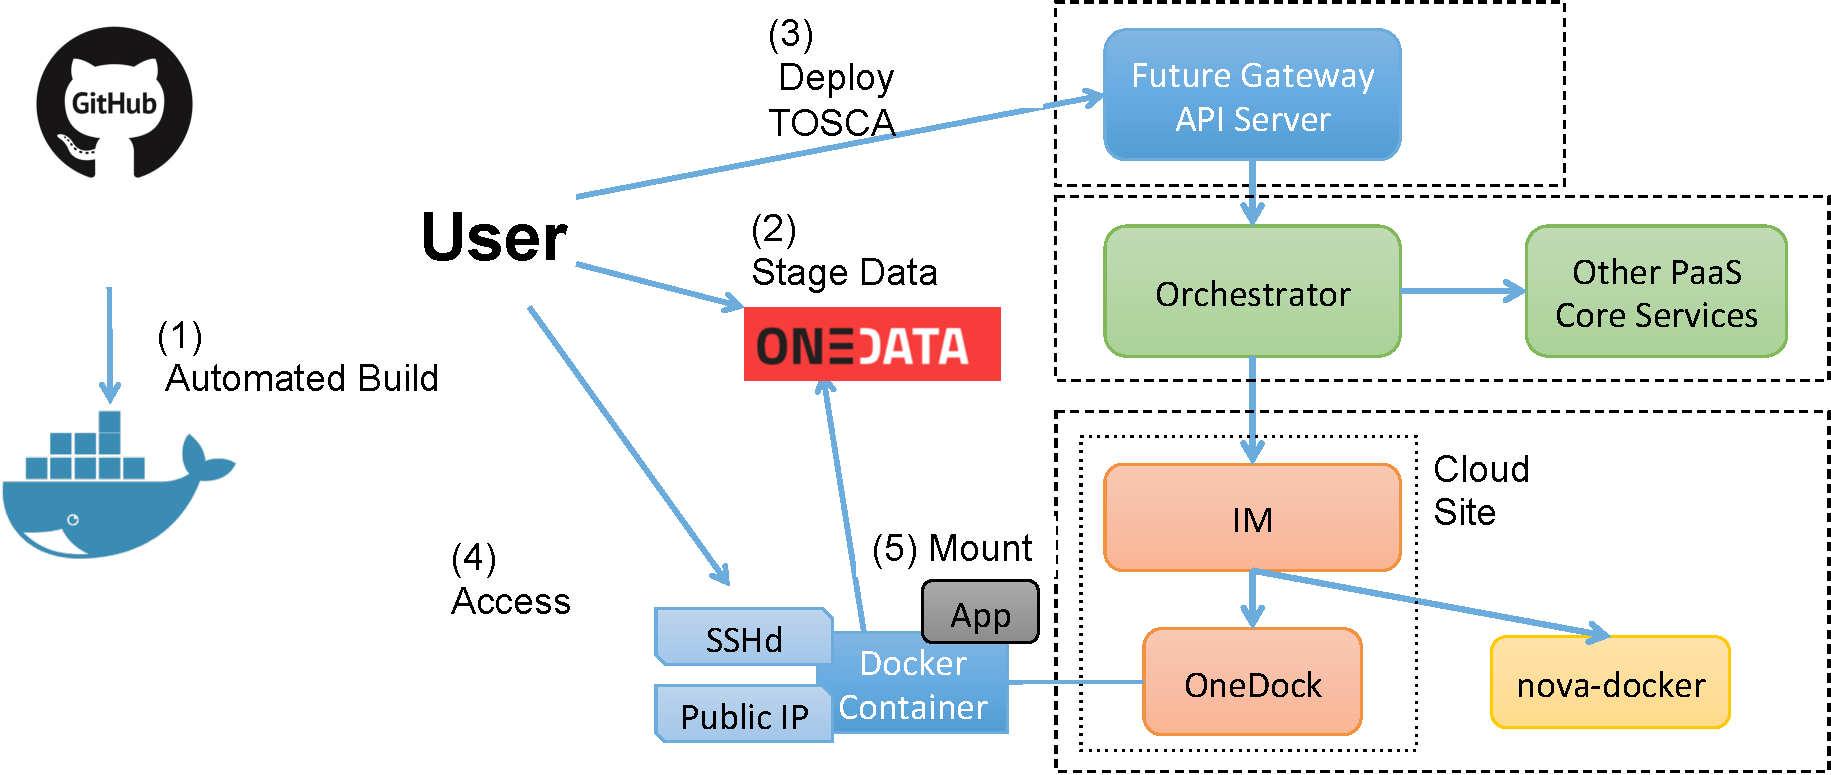
\includegraphics[width=\textwidth]{./figs/Figure12.pdf}
  \caption{Basic execution of containers using INDIGO solutions}
  \label{fig:12}
\end{figure}



\subsection{Building advanced applications using INDIGO solutions}


In this section, we present several simplified schemes, corresponding to different applications already implemented, with the idea that they can be more easily used as a guide to configure new applications.  

The key, as stated before, is the composition of the template, written using the TOSCA language, specifying:

\begin{itemize}
\item the image of the application to be used, as a container, using docker technology.
\item the resources (CPUs, storage, memory, network ports) required to support the execution
\item the parameters required to configure INDIGO services used like, for example, OneData
\item idem for additional cloud services (like Mesos/Marathon)
\end{itemize}
Examples of TOSCA templates can be found at https://github.com/indigo-dc/tosca-templates FutureGateway offers a friendly way to handle the TOSCA templates to launch the applications.

\begin{itemize}
\item A first example is the deployment, as a SaaS solution, of a digital repository. The scheme is presented in the Figure \ref{fig:13} below. The specific template for this application is available for reuse in the github repository of the project.

The repository manager, controlling the application, uses the FutureGateway to configure the application, based on the ZENODO software, that can be automatically scaled up and ensure its high availability using Cloud resources as needed, and also enabling the authentication and authorization mechanism  for their research community, DARIAH, based on the INDIGO solution IAM. 

All these details are transparent to the final user, who accesses the repository directly through its web interface, and benefits of the enhanced scalability and availability.



\begin{figure}
  \centering
  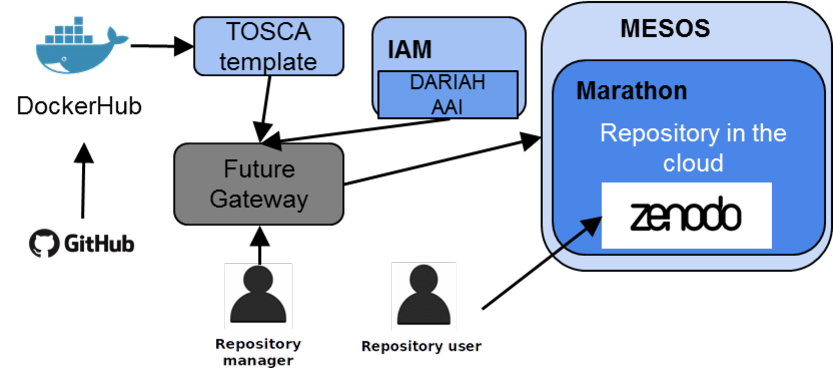
\includegraphics[width=\textwidth]{./figs/Figure13.pdf}
  \caption{Deployment of a digital repository using INDIGO solutions}
  \label{fig:13}
\end{figure}



\item A second example is the launch of a Virtual Elastic Cluster to support a data intensive system.The scheme is presented in Figure \ref{fig:14} below. 

The specific template for this advanced application is available for reuse in the github repository of the project.

Galaxy is an open source, web-based platform for data intensive biomedical research. This application deploys a Galaxy instance provider platform, allowing to fully customize each virtual instance through a user-friendly web interface, ready to be used by life scientists and bioinformaticians.

The front-end that will be in charge of managing the cluster elasticity can use a specified LRMS (selected among torque, sge, slurm and condor) workload.

All these details are transparent to the final user, the researcher, who accesses the Galaxy instance directly through its web interface, and benefits of the enhanced scalability and availability.

This complex template includes the configuration of the distributed storage based in OneData, the use of the encrypted files via LUKS, the deployment of elastic clusters using another INDIGO solution, CLUES, and the integration of the Authentication and Authorization mechanism, very relevant for this application area, using IAM.  

\begin{figure}
  \centering
  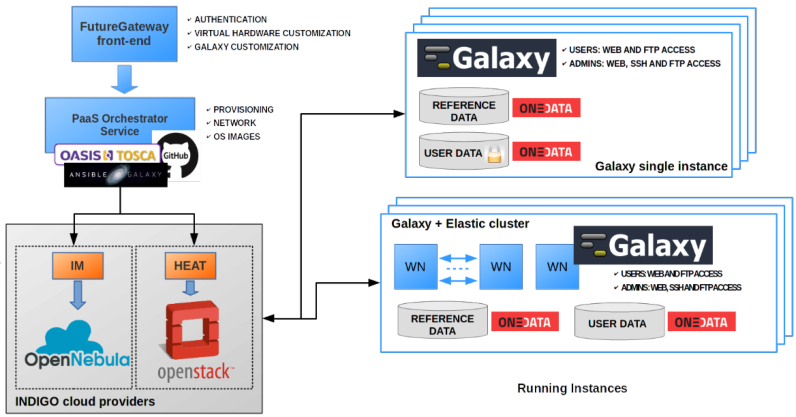
\includegraphics[width=\textwidth]{./figs/Figure14.pdf}
  \caption{Launching of a Virtual Elastic Cluster using INDIGO solutions}
  \label{fig:14}
\end{figure}



\end{itemize}





\section{Conclusions}
\label{sec:conclusions}

Thanks to the new common solutions developed by the INDIGO project, teams of first-line researchers in Europe are using public and private Cloud resources to get new results in Physics, Biology, Astronomy, Medicine, Humanities and other disciplines. 

INDIGO-developed solutions that have for instance enabled new advances in understanding how the basic blocks of matter (quarks) interact, using supercomputers, how new molecules involved in life work, using GPUs, or how complex new repositories to preserve and consult digital heritage can be easily built. The variety of the requirements coming from these so diverse user communities proves that the modular INDIGO platform, consisting of several state-of-the-art, production-level services, is flexible and general enough to be applied to all of them with the same ease of use and efficiency. 

These services allow to federate hybrid resources, to easily write, port and run scientific applications to the cloud. They are all freely downloadable as open source components, and are already being integrated into many scientific applications, namely: 

\begin{itemize}
\item High-energy physics: the creation of complex clusters deployed on several Cloud infrastructures is automated, in order to perform simulation and analysis of physics data for large experiments. 
\item Lifewatch: parameters from a water quality model in a reservoir are calibrated, using automated multiple simulations. 
\item Digital libraries: multiple libraries can easily access a cloud environment under central coordination but uploading and managing their own collections of digital objects. This allows them to consistently keep control of their collections and to certify their quality. 
\item Elixir: Galaxy, a tool often used in many life science research environments, is automatically configured, deployed on the Cloud and used to process data through a user-friendly interface. 
\item Theoretical HEP physics: the MasterCode software, used in theoretical physics, adopts INDIGO tools to run applications on Grids, Clouds and on HPC systems with anefficient, simple-to-use, consistent interface. 
\item In DARIAH, a pan-european social and technical infrastructure for arts and humanities, the deployment of a self-managed, auto-scalable Zenodo-based  repository in the cloud is automated. 
\item Climate change: distributed, parallel data analysis in the context of the Earth System Grid Federation (ESGF) infrastructure is performed through software deployed on HPC and cloud environments in Europe and in the US. 
\item Image analysis: in the context of EuroBioImaging, a distributed infrastructure for microscopy, molecular and medical imaging, INDIGO components are used to perform automatic and scalable analysis of bone density. 
\item Astronomical data archives: big data consisting of images collected by telescopes are automatically distributed and accessed via INDIGO tools. 
\end{itemize}

The same solutions are also being explored by industry, to provide innovative services to EU companies: for example, modelling water reservoirs integrating satellite information, improving security in cyberspace, or assisting doctors in diagnostics through medical images. 

The outcomes of INDIGO-DataCloud will persist, and also be extended, after the end of the project because. INDIGO was one of the three coordinating projects (together with EGI and EUDAT) in the preparation of the EOSC-hub proposal submitted to the EC H2020 EINFRA-12 call; the main goal of this recently approved project is to contribute to the EOSC implementation by enabling seamless and open access to a system of research data and services provided across nations and multiple disciplines. 

Many INDIGO components will find place in the unified service catalogue provided by EOSC-hub. In addition INDIGO nominates the Technology Coordinator of the entire project, in recognition of the impressive work we have been doing in these 30 months. 

Two additional Horizon 2020 projects were also approved ({\tt DEEP HybridDataCloud} and {\tt eXtreme DataCloud}), that will continue to develop and enhance INDIGO components to provide new and exciting innovative services. 

INDIGO solutions are also being intensively tested in other projects, such as HelixNebula ScienceCloud. To conclude, the 30 months of the INDIGO-DataCloud project were totally exciting and ripe with results, well beyond what was originally foreseen. We believe that the foundations laid by INDIGO will continue to find proper development and adoption in a wide variety of fields, public and private, at the service of science and for the benefit of the overall general public.  

\section*{Acknowledgments}
INDIGO-Datacloud has been funded by the European Commision H2020 research and innovation program under grant agreement RIA 653549. 

\bibliography{references}
\bibliographystyle{unsrt}


\section*{Appendix}

The processes and procedures implemented in our software management activity have facilitated contributions and merge in upstream projects.
Here follows the list of software developed in the framework of INDIGO-Datacloud that has been contributed upstream to the Open Source community.


\begin{itemize}

\item OpenStack (https://www.openstack.org) 
\begin{itemize}
\item Nova Docker
\item Heat
\item OpenID-Connect for Keystone
\item Pre-emptible instances support (under discussion)
\item OCCI implementation for OpenStack (https://github.com/openstack/ooi) 
\end{itemize}
\item OpenNebula (http://opennebula.org) 
\begin{itemize}
\item OneDock
\item Patch to support FaSS
\item Extended AWS support for rOCCI in OpenNebula. Python and Java libraries for OCCI support.
\end{itemize}
\item Infrastructure Manager (http://www.grycap.upv.es/im/index.php)
\item Clues (http://www.grycap.upv.es/clues/eng/index.php)
\item Onedata (https://onedata.org) 
\item Apache Libcloud (https://github.com/apache/libcloud)
\item Kepler Workflow Manager (https://kepler-project.org/)

\item TOSCA adaptor for JSAGA (http://software.in2p3.fr/jsaga/dev/) 

\item CDMI and QoS extensions for dCache (https://www.dcache.org) 
\item Workflow interface extensions for Ophidia (http://ophidia.cmcc.it) 
\item OpenID Connect Java implementation for dCache (https://www.dcache.org) 
\item MitreID (https://mitreid.org/) and OpenID Connect (http://openid.net/connect/) libraries
\item FutureGateway (https://www.catania-science-gateways.it/)

\end{itemize}



\end{document}


